\documentclass{scrreprt}
\setcounter{secnumdepth}{5}
\usepackage{graphicx}
\usepackage[utf8]{inputenc}
\usepackage{tikz}
\usepackage{listings}
\usepackage{underscore}
\usepackage[bookmarks=true]{hyperref}
\usepackage{placeins}
\usepackage{caption}
\hypersetup{
    bookmarks=false,    % show bookmarks bar?
    pdftitle={Software Requirement Specification},    % title
    pdfauthor={Yiannis Lazarides},                     % author
    pdfsubject={TeX and LaTeX},                        % subject of the document
    pdfkeywords={TeX, LaTeX, graphics, images}, % list of keywords
    colorlinks=true,       % false: boxed links; true: colored links
    linkcolor=blue,       % color of internal links
    citecolor=black,       % color of links to bibliography
    filecolor=black,        % color of file links
    urlcolor=purple,        % color of external links
    linktoc=page            % only page is linked
}%
\def\myversion{1.4}
\date{}
\usepackage{hyperref}
\begin{document}
\begin{titlepage}
  \flushright\bfseries\huge
  \vspace*{\stretch{0.4}}
    \rule{\linewidth}{5pt}
    \par
    \vspace{1cm}
    {\Huge DESIGN \par DOCUMENT \par}
    \vspace{2cm}
    for \\
    \vspace{2cm}
    Personal Dietary Application \\
    \vspace{2cm}
     \LARGE{Version \myversion \\}
    \vspace{2cm}
    by Craig Boucher \\
    Md Tanveer Alamgir \\
    Fan Zou\\
    Osman Momoh \\
    Xin Ma
    \vspace{2cm}
    \rule{\linewidth}{5pt}
    \vspace{\stretch{1}}
\end{titlepage}
\tableofcontents
\chapter{Introduction}
The project undertaken in this COMP 5541 course involves creating an application that keeps track of dietary records for the user. This diet application has been designed to use the border pane layout for the main window of the User Interface (UI). \\ \\ 
This design document will provide details for the type of software architecture used to develop the software and explain the design for the user interface. The architectural component illustrates the abstraction of the software classes involved and how they relate to each other to manipulate and process data that the user interacts with. The interface design section will assess the process for the states the user goes through to interact with the personal dietary application.
\section{Purpose}
This document will serve as an illustration for the architectural design choices as well as an explanation for the properties of the user interface implemented for the Personal Dietary Application software. This software project is being completed for the COMP 5541 graduate diploma course at Concordia University. There will be diagrams to showcase the type of the architecture used and a domain diagram which encompasses real world concepts to work from and aid in designing the software. Screenshots are used to provide a valuable perspective on the user interface. These graphical aids are described in further detail to demonstrate the functionality of the interface.
\section{Scope}
In order to provide proper design documentation for the Personal Dietary Application this document will be properly formatted and includ all necessary information. The team responsible for surveying this document and creating the software will be able to use the robust explanation of the architectural model presented in this document to carry out the necessary work. The visual graphics demonstrating the user interface design choices will serve as a guide for the team to orchestrate the proper performance of the software.
\section{Definitions and Abbreviations}
\subsection{Definitions}
\begin{tabular}{|l|l|}
\hline
	Term & Definition \\
\hline
	Model View & Software architecture that renders funcionality between three components. \\
	Controller & The view is the user interface. The model stores the data and the controller \\
	& mediates data transfer between the view and model. \\
\hline
	Date & Allows user to enter day and month of an entry for an item. \\
\hline
	Consumed & The user will be able to mark a food item as consumed (eaten) or not. \\
\hline
\end{tabular}

\subsection{Abbreviations}
\begin{tabular}{|l|l|}
\hline
	Abbreviation & Term \\
\hline
	MVC & Model View Controller \\
\hline
	GUI & Graphical User Interface \\
\hline
	UML & Unified Modeling Language \\
\hline
	PDA & Personal Dietary Application \\
\hline
	GRASP & General Responsibility Assignment Software Patterns \\
\hline
\end{tabular}

\section{References}
https://upload.wikimedia.org/wikipedia/commons/a/a0/MVC-Process.svg \\
http://users.encs.concordia.ca/~paquet/wiki/images/e/ee/Phase2final.pdf
\section{Overview}
Following the introduction, the remaining portions of the document is composed of three main sections. First, there is a section dedication to Architectural Design. Second, the largest section, consists of Software Interface Design. In the portion concerning the software architecture the three smaller sections are related to the reasoning for choosing the architecture, a diagram illustrating how the architecture behaves abstractly, and the closing architectural section details how software files will operate together on the computer. \\
The interface section will provide documentation regarding the system, modules, and dynamic interfaces for the software project. \\
The final section consists of state sequence diagrams. These diagrams showcase the inner method call sequence and the different states the software application will traverse in order to fulfill user operations.
\chapter{Architectural Design}
\section{Rationale}
The Model View Controller (MVC) architecture design pattern has been chosen for this software project. Model, View, and Controller are the three components which comprise this architecture. \\

The purpose of the Controller model is to navigate and facilitate the transfer of data between the View and the Model. The Controller is responsible for acquiring data input from the user, manipulate the model with the necessary memory changes, and provide updates to the View if and when exceptions or errors are thrown. \\

The View is where the (graphical) user interface rests. The information stored in the model is used by the View to display everything necessary to the user. Everything the user interacts with rests with the View, from input functionality to button objects. Whenever data is manipulated in the Model the View will reflect this accordingly, adhering to the Observer software design pattern. \\

The objective of the Model is to store all of the necessary information and data that the application requires to operate successfully. All of the data is stored in local memory. Every food item and all of the details of each item is stored in the Model module. There is a list of every food item added by the user that is stored in the Model (Observable List), and whenever a change is made (adding or removing food items), the View will graphically respond to these changes. \\

\begin{figure}[!htbp]
\centering
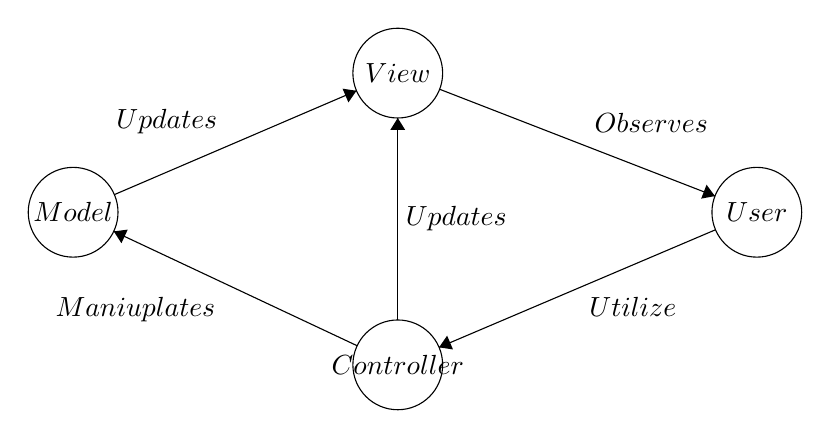
\begin{tikzpicture}[scale=0.19]
\tikzstyle{every node}+=[inner sep=0pt]
\draw [black] (39.5,-15.1) circle (3);
\draw (39.5,-15.1) node {$View$};
\draw [black] (17.8,-24.4) circle (3);
\draw (17.8,-24.4) node {$Model$};
\draw [black] (39.5,-34.6) circle (3);
\draw (39.5,-34.6) node {$Controller$};
\draw [black] (63.5,-24.4) circle (3);
\draw (63.5,-24.4) node {$User$};
\draw [black] (42.3,-16.18) -- (60.7,-23.32);
\fill [black] (60.7,-23.32) -- (60.14,-22.56) -- (59.78,-23.49);
\draw (56.44,-19.14) node [above] {$Observes$};
\draw [black] (60.74,-25.57) -- (42.26,-33.43);
\fill [black] (42.26,-33.43) -- (43.19,-33.57) -- (42.8,-32.65);
\draw (55.21,-30.05) node [below] {$Utilize$};
\draw [black] (36.78,-33.32) -- (20.52,-25.68);
\fill [black] (20.52,-25.68) -- (21.03,-26.47) -- (21.45,-25.56);
\draw (21.96,-30.05) node [below] {$Maniuplates$};
\draw [black] (20.56,-23.22) -- (36.74,-16.28);
\fill [black] (36.74,-16.28) -- (35.81,-16.14) -- (36.2,-17.06);
\draw (24.06,-19.19) node [above] {$Updates$};
\draw [black] (39.5,-31.6) -- (39.5,-18.1);
\fill [black] (39.5,-18.1) -- (39,-18.9) -- (40,-18.9);
\draw (40,-24.85) node [right] {$Updates$};
\end{tikzpicture}
\caption{Diagram of MVC architecture and Observer design pattern}
\end{figure}

The software specifications outlined in the project instructions specifically mandated the MVC architecture. The purpose of this architecture is to provide a relevant abstraction of how desktop, mobile, or web applications operate when requiring constant use by a user. The abstraction allows three distinct modules to operate independently of each other and be capable of being updated separately. Different developers can be assigned to develop for the various modules with minimal cooperation required between them as the core functionality of each module remains the same across updates.

\section{Software Architecture Diagram}

An abstract depiction of the MVC architecture is illustrated in the below figure. The User actor will use the controller to manipulate the model. In turn, the model provides updates to the View that the user is observing.

\begin{figure}[ht]
\centering
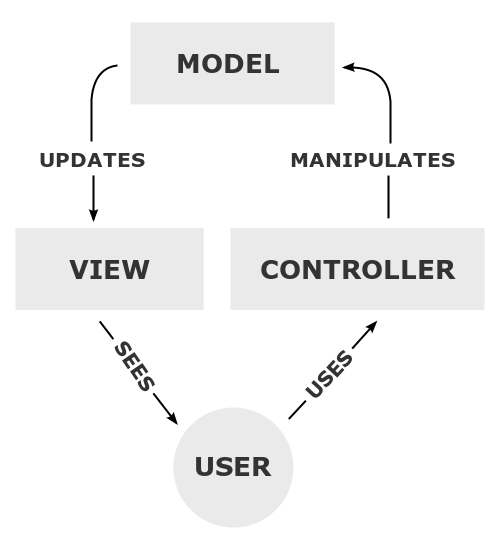
\includegraphics[height=9cm]{pictures/MVC-Process.png}
\caption{Source for image found under section 1.4}
\end{figure}

The graphical user interface (GUI) that the user witnesses and interacts with is contained in the View module. The user can keep track of the dietary items they add to the application with the provided graphical display window. The user also has the option to remove these dietary items. The noted food groups that have been consumed are also indicated in this UI window. \\

The model is the core module of the system. Every piece of data input by the user is stored in the model under local memory. When the appropriate changes are made to the data contained in the model the View is updated as needed. The application relies on the model to relay accurate data to the user through the View. \\

The controller contains all of the necessary logic to provide additional data to the model and modify any existing data as required. The user will use their I/O peripherals (mouse, keyboard) to input data into text fields or click the various button options available to interact with the controller.

\subsection{Observable Model \& Observing View}

\begin{figure}[ht]
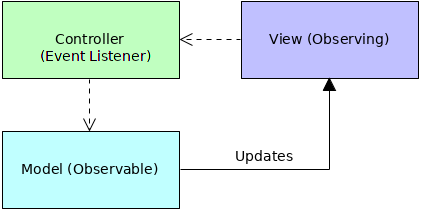
\includegraphics[width=10cm]{pictures/obsv2.png}
\caption{Diagram of the Observer-Model design.}
\end{figure}

The above diagram illustrates the link between the Model component and the View component. The previous sections of this document discussed the MVC (Model-View-Controller) architecture and the overall operation between all three components. However, it is important to note that the software project described by this design document combines the Observer pattern with the MVC pattern. The personal dietary application makes use of events when responding to user input. These events are responded to by the Controller which manages the transfer of data to the Model. Once this data is stored successfully the Model performing the Observable functionality will provide updates to the Observing View of all state changes that occur.

\section{System Topology}

The personal dietary application is developed with the Java programming language. Therefore, the executable .jar file will be runnable on a variety of hardware. Online communication is not required to run the application. In the current iteration, only local memory is used to store the user data. There are plans to implement a local database as well.

\chapter{Software Interface Design}
\section{System Interface Diagrams}

Our personal dietary application has only system level interface. The application does not employ any software or hardware interfaces. GUI is the system level interface. GUI allows the user to interact with the application. By using the GUI the user will be able to add a food item, mark it as eaten or not eaten, hide an added item, remove an item and provide updates to the list keeping track of the various dietary items.

\subsection{User Interface}

The user will interact with the software using the user interface. An attempt was made to make it as user friendly as possible by placing the components with an order of their importance and utilizing the full screen mode. Below are a few points taken into consideration for the user interface:

\begin{itemize}
\item User Friendly: Making it user friendly by putting important components according to the user's view point.
\item Easy to find information: Since the application is all about their dietary needs, so it was important to make it easy to calculate and display their consumed and need to consumed items. It was made as handy as possible.
\item Guiding user: Guiding user by displaying different colour if they miss out something while inputting a food item.
\end{itemize}

\subsection{Interface Description}
The system interfaces that establishes the interaction between user and computer are described below:

\clearpage

\subsection{Landing page}
Below is the first screen that the user will see when they will launch the application. Here is the description of every option available to user:

\begin{figure}[!htbp]
\centering
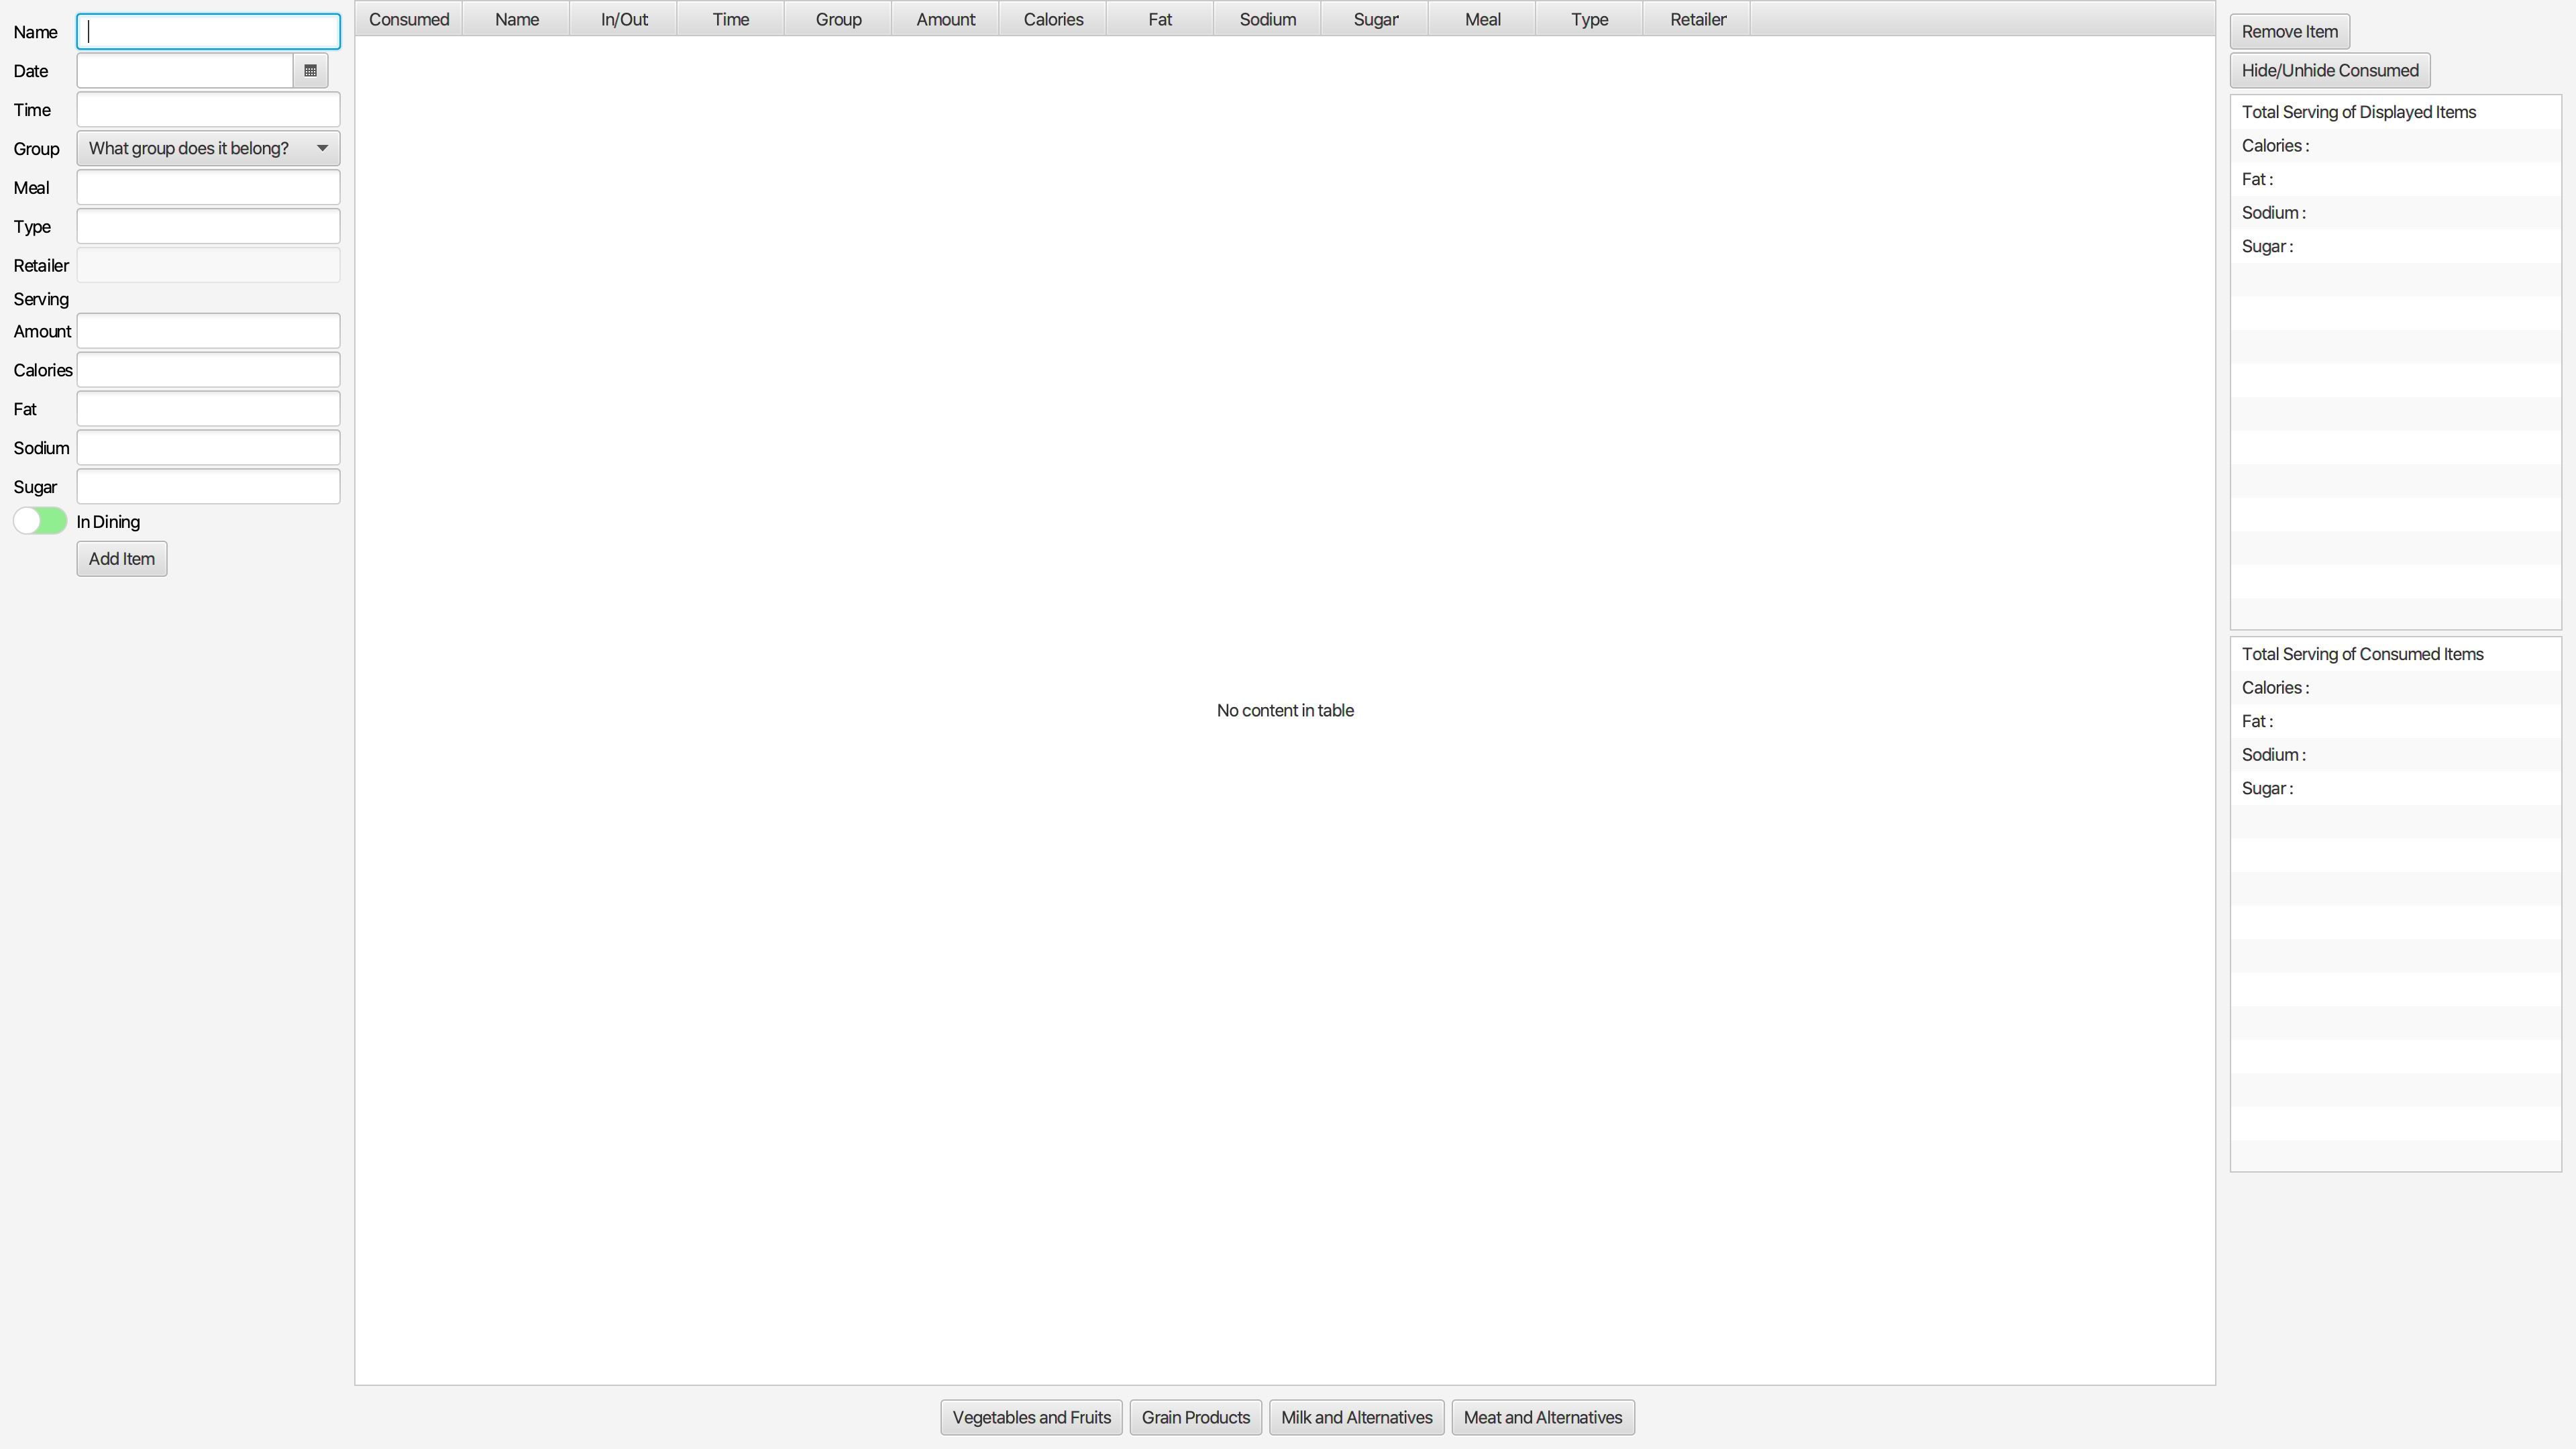
\includegraphics[width=15cm]{pictures/raw.png}
\caption{Landing page}
\end{figure}
\FloatBarrier
\begin{enumerate}
\item Add a food item: User can input the food details to have it added.
\item Display the added food: It is a list of all food added by user
\item Remove a food item: It is a button to remove a food item from added list.
\item Hide/unhide Consumed food: This button gives the user ability to hide/unhide consumed food.
\item Total serving: It will show the total serving of all the items in the added food list.
\item Serving of consumed item: This will only show the total serving of consumed item(s).
\item Food group: Based on the food item(s) added and consumed these 4 button will indicate which group they belong to.
\end{enumerate}
	
\subsection{Add Food Item Scenario}

Below gives the ability for the user to add a food item by inserting the details of the food:

\begin{figure}[!htbp]
\centering
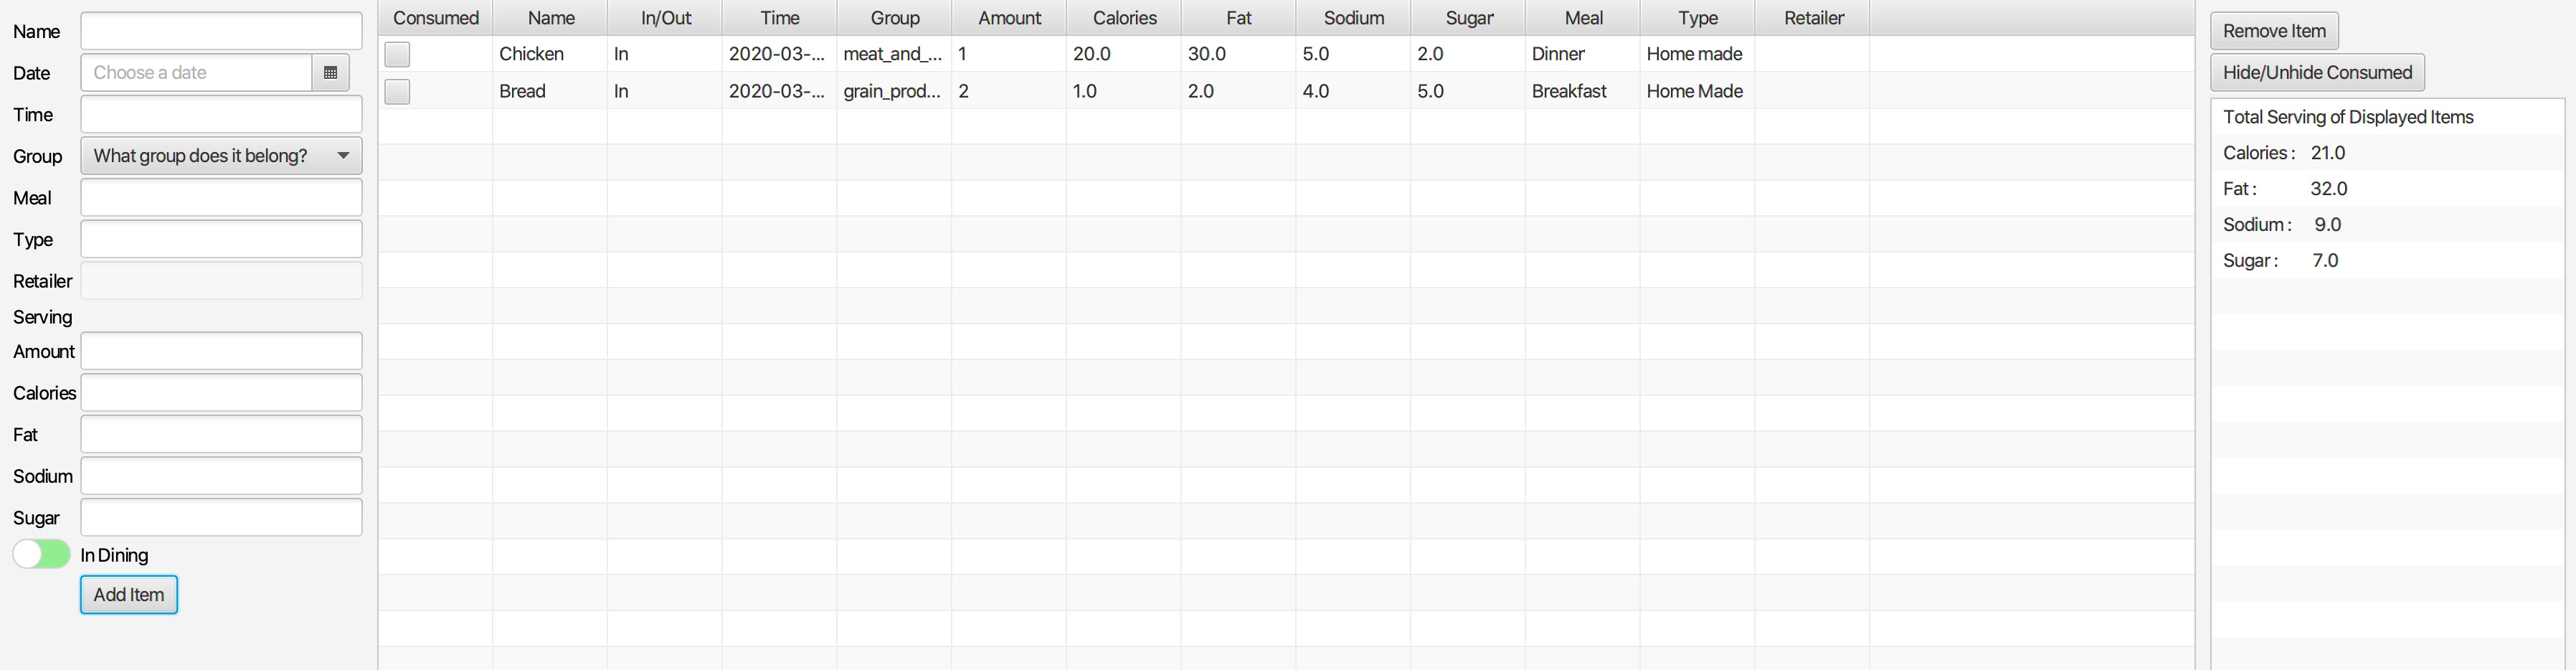
\includegraphics[width=15cm]{pictures/add-food-item.png}
\caption{Add a food item}
\end{figure}

\FloatBarrier

\begin{enumerate}
\item Name: User will insert the name of the food.
\item Date: User will select the date from the calendar on the right side of the text box.
\item Time: User will insert the time of the food consumed. Time the is in 24h format.
\item Food Group: User will select the respective food group from the drop down menu.
\item Meal: User will insert the meal they consumed the food at.
\item Type: This field is for user to indicate whether the food was bought, homemade. If the food was consumed at out dining then this field will get greyed out.
\item Retailer: This is to identify the name of the retailer if the food was consumed from out dining. If in dining is selected using the toggle switch at the bottom then this field will be greyed out.
\item Amount: The amount of food consumed by the user.
\item Calories: The amount of calories presented in the consumed food.
\item Fat: The amount of fat presented in the consumed food.
\item Sodium: The amount of Sodium presented in the consumed food.
\item Sugar: The amount of Sugar presented in the consumed food.
\item Toggle Switch (In dining/Out Dining): This toggle switch will allow the user to choose whether the food was consumed inside of outside.
\item Add Item: After Filling out all the details of the food, the user will press the Add Item button to add the food item.
\item Validation: If the user does not fill out all the fields then the placeholder will show up to indicate which field needs to be filled out and what to put inside that field.

\begin{figure}[!htbp]
\centering
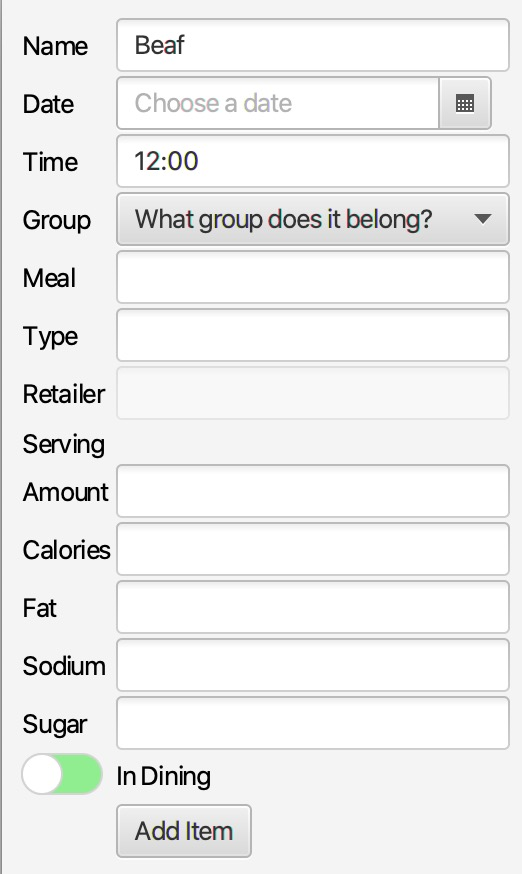
\includegraphics[width=5cm]{pictures/err-add-item.png}
\caption{Validation of input}
\end{figure}

\FloatBarrier
\end{enumerate}

Once a food item has been added successfully the details will show up on the list section at the middle of the page. As we keep on adding food items on the very left side the total serving will be calculated. This serving is not for consumed item(s), this is the total of all the food items added by the user.
\pagebreak
\subsection{Set Food Item as Consumed Scenario}

\begin{figure}[!htbp]
\centering
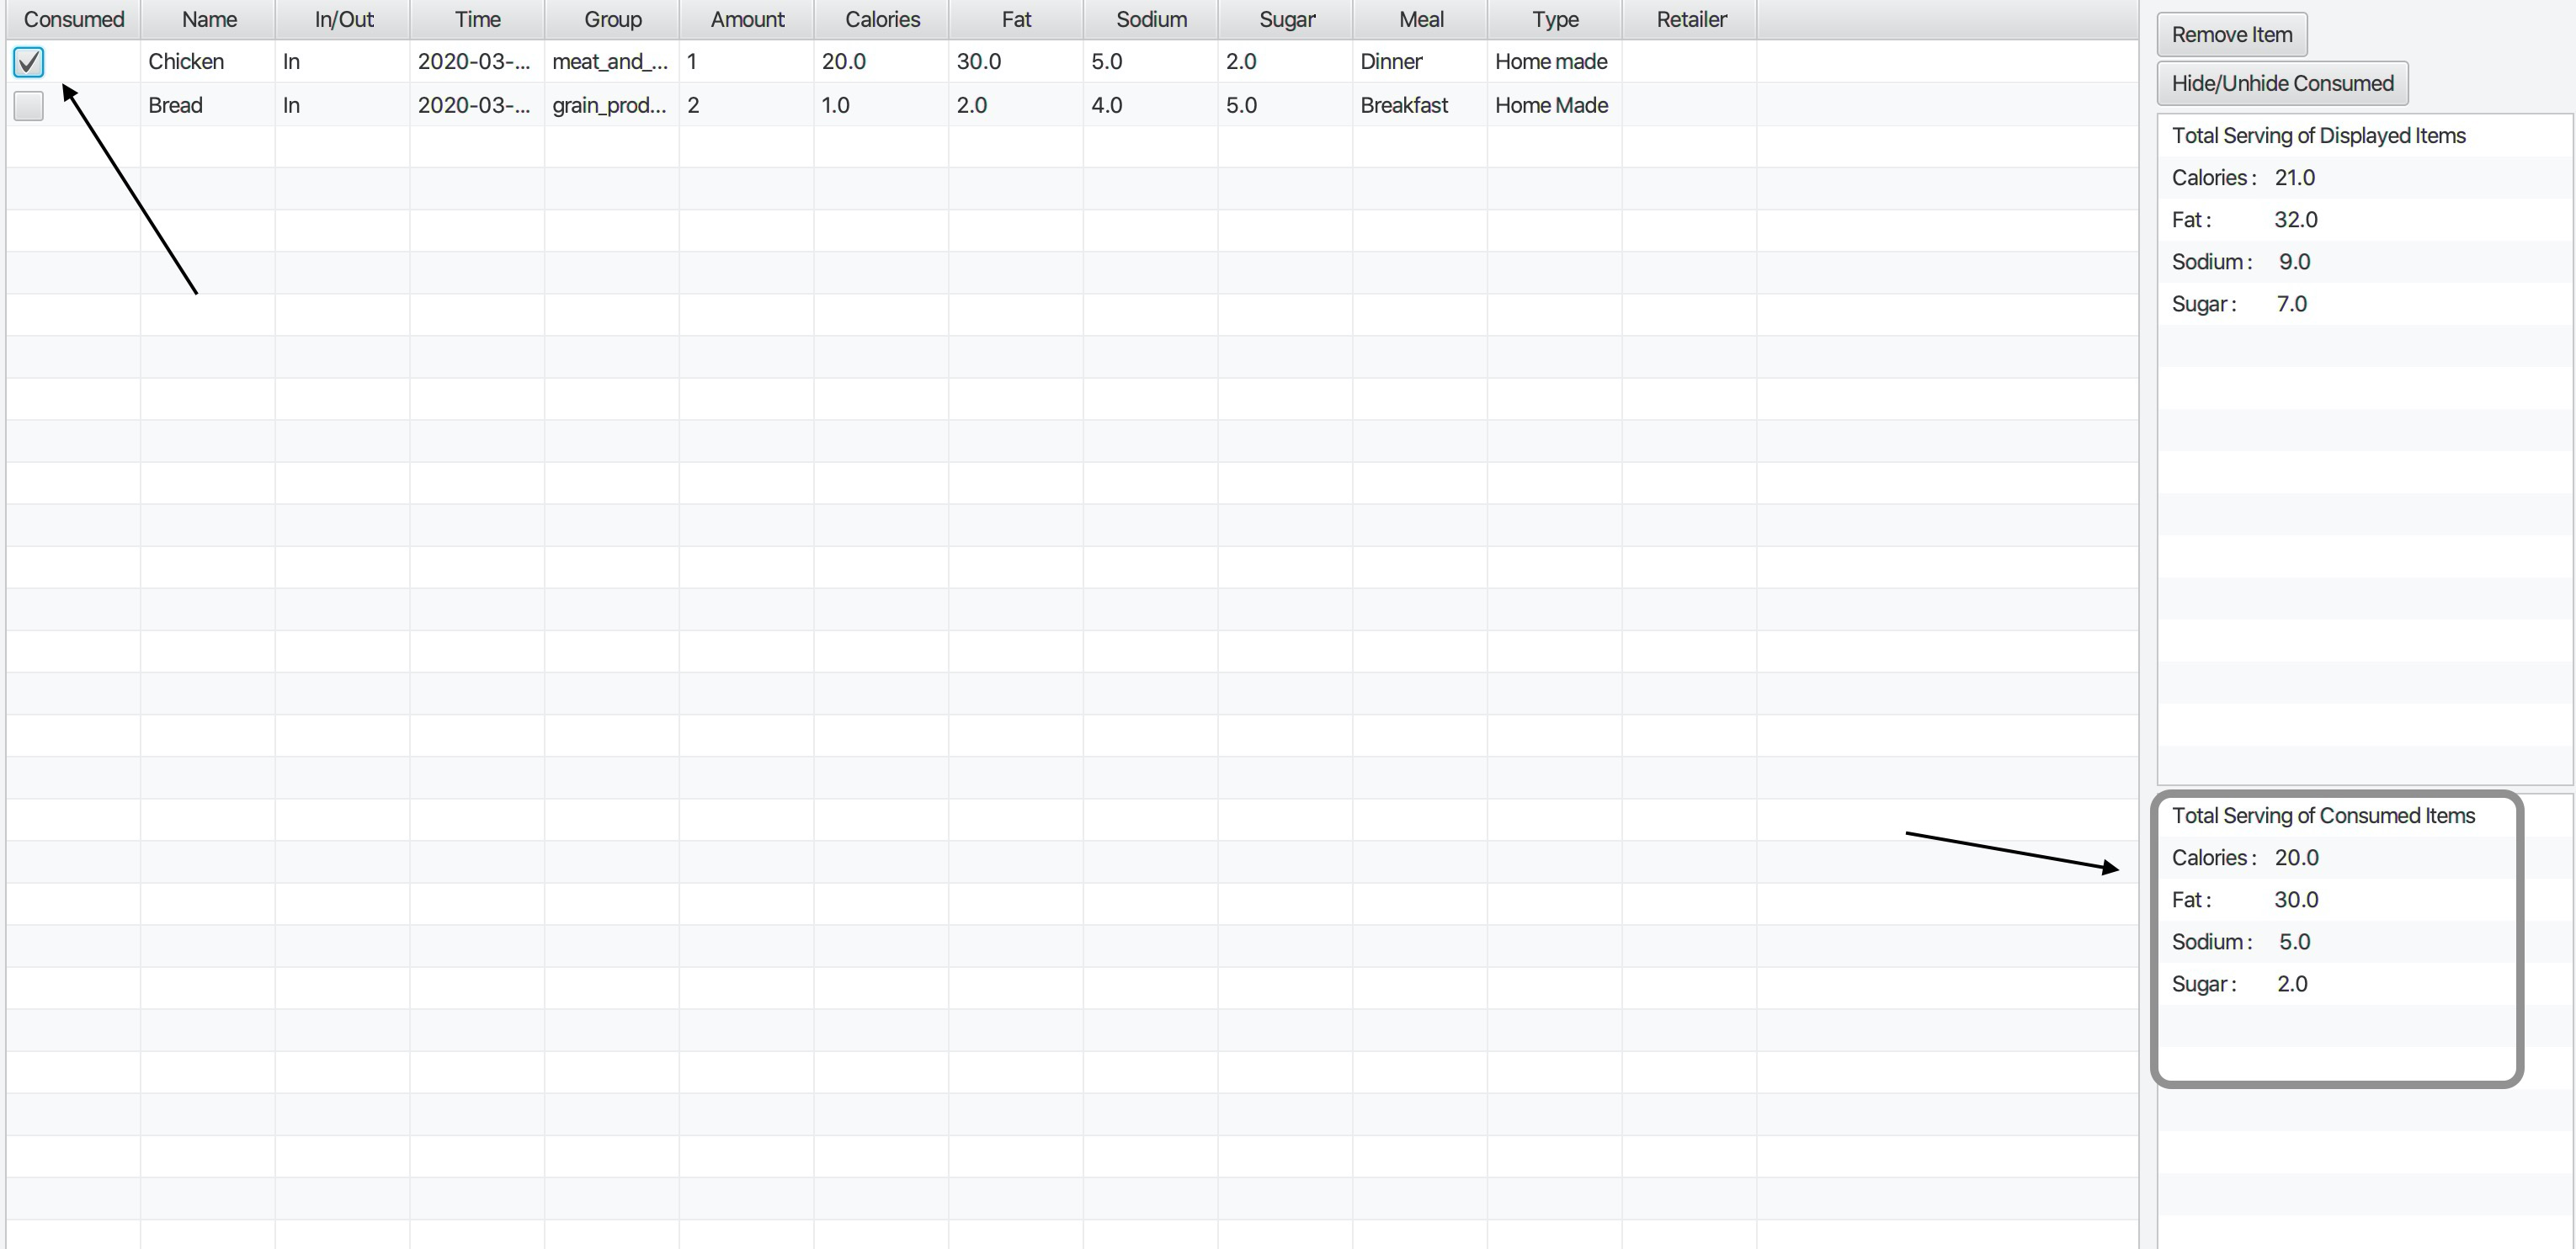
\includegraphics[width=15cm]{pictures/consumed.png}
\caption{Mark as consumed}
\end{figure}

\FloatBarrier

In the display list of the food item(s) the user will have the option to mark a food as consumed by clicking the checkbox in "Consumed" column. As the user keeps on marking different food items as consumed from display list the total serving (Total serving of consumed list) will be changing on the left side.

\subsection{Set Food Item as Unconsumed Scenario}

If a food item has been marked as consumed, the user has the option to click on the checkbox again of the same food item to remove the mark and mark it as unconsumed. After making a food item as unconsumed the serving of that particular food will be deducted from the "Total serving of consumed food".

\subsection{Remove Food Item Scenario}

\begin{figure}[!htbp]
\centering
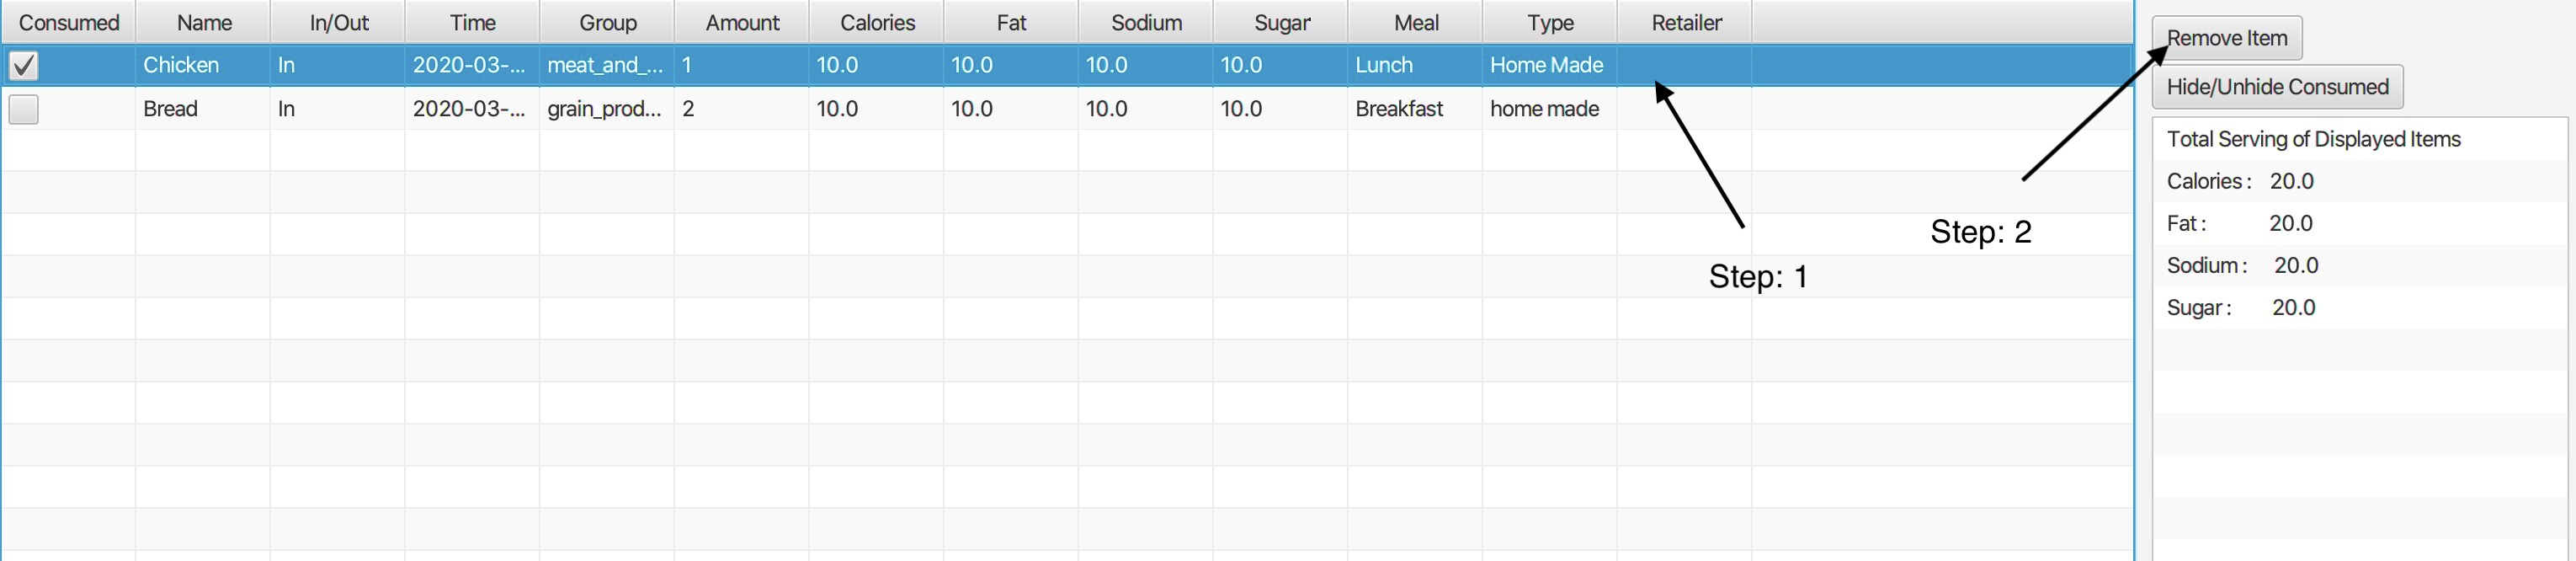
\includegraphics[width=15cm]{pictures/remove-food.png}
\caption{Remove a food item}
\end{figure}

\FloatBarrier

To remove a food item there are two steps the user needs to follow:

\begin{enumerate}
\item Step 1: First, the user needs to select the item he/she wants to remove from the display list.
\item Step 2: Then they need to click the remove button.
\end{enumerate}

\subsection{Hide Consumed Diet Scenario}

\begin{figure}[!htbp]
\centering
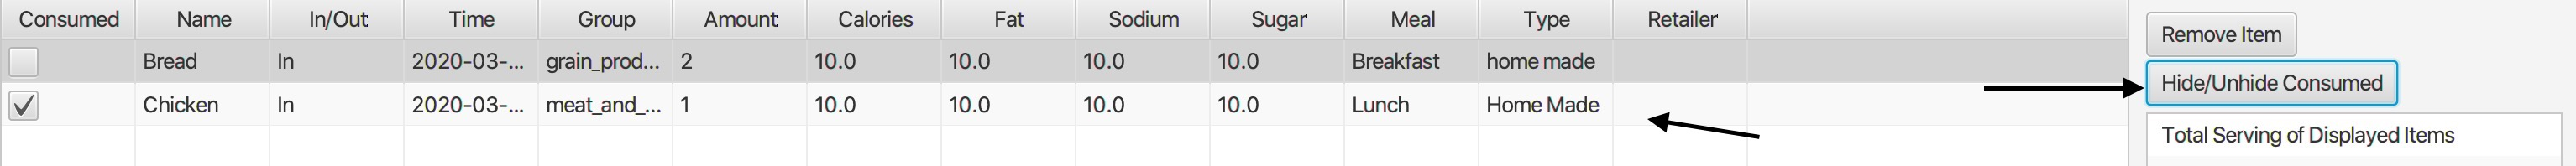
\includegraphics[width=15cm]{pictures/hide.png}
\caption{Hide consumed item(s)}
\end{figure}

\FloatBarrier

When the user clicks the "Hide/Unhide Consumed" button on the right had side all the consumed food item(s) will disappear from the display list. It also updates the "Total serving of displayed items" as this list displays the serving of all displayed food items.

\subsection{Unhide Consumed Diet Scenario}

When all the item(s) are hidden by a user then the user can click the same "Hide/Unhide Consumed" button again to make all the consumed food item(s) appear on the display list. Also the "Total serving of displayed items" list will be updated.

\pagebreak

\subsection{Marking food Group}

\begin{figure}[!htbp]
\centering
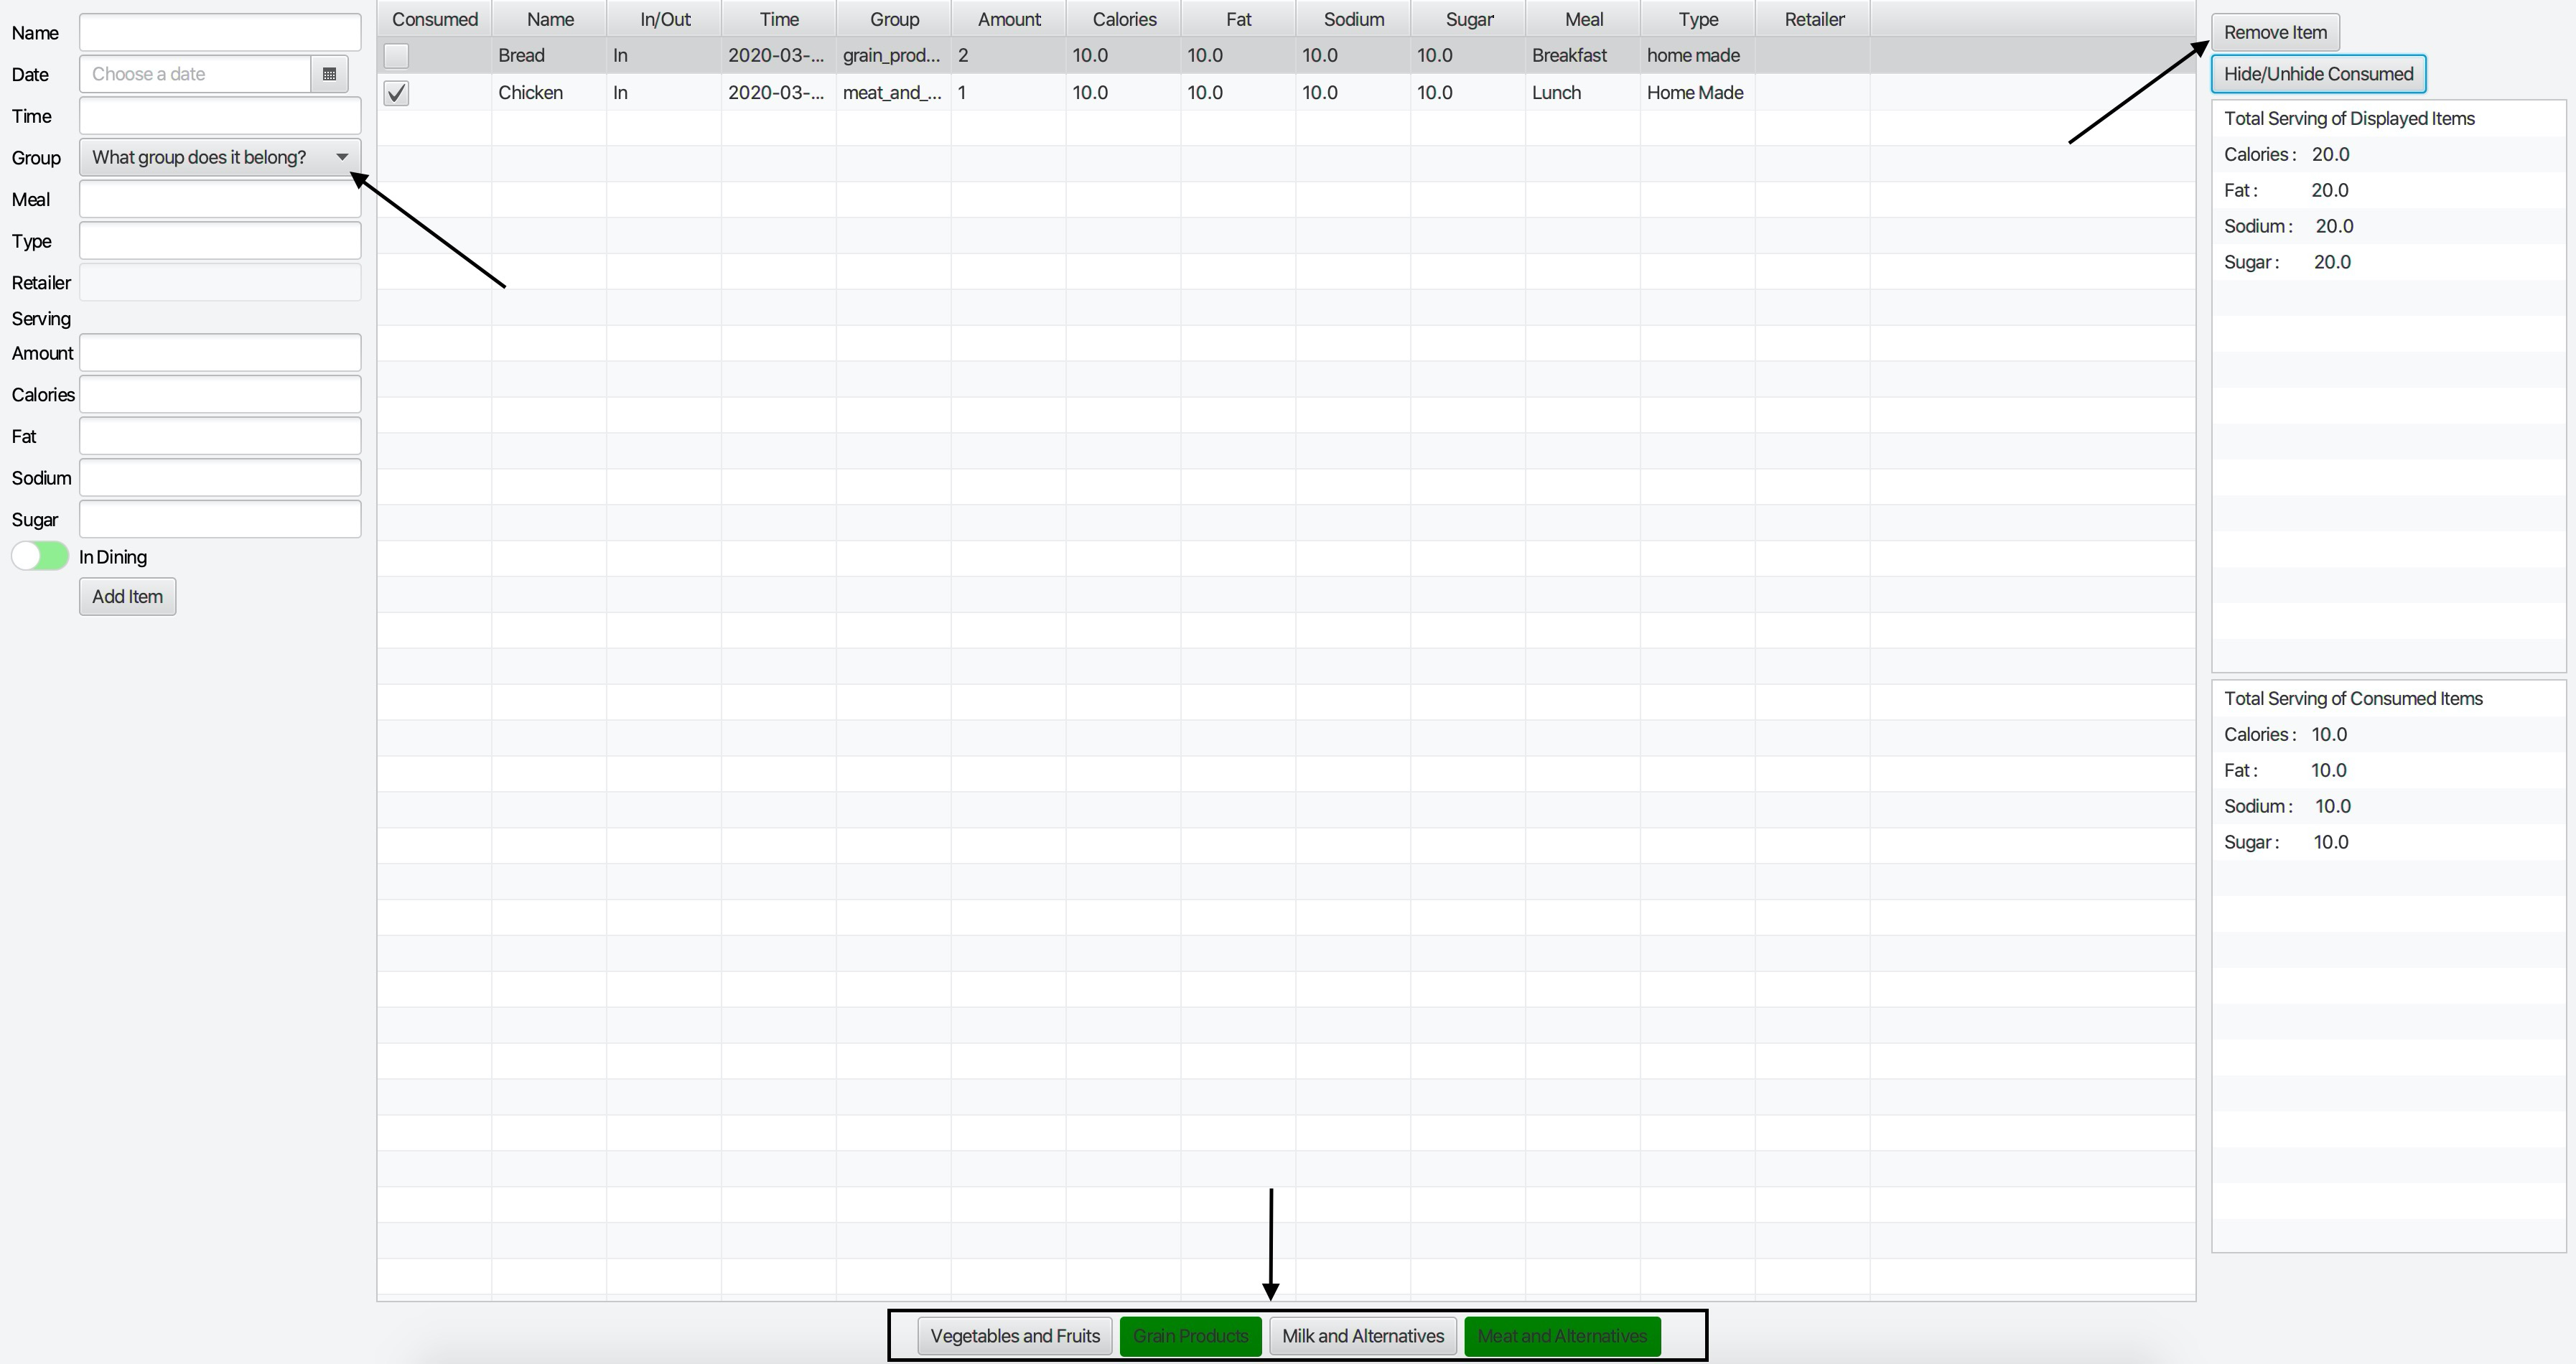
\includegraphics[width=15cm]{pictures/food-group.png}
\caption*{Marking good group}
\end{figure}

\FloatBarrier

To mark a food group the user does not need to do anything explicitly. During the adding of a food item they need to select a food group from drop down. Once a food group has been selected and added in the display list the respective food group will light up in green colour. On the other hand if the user removes a food item from the display list and there is no food item present of a particular food group in the display list then that food group will set back to grey colour indicating there is no food present in the list of that food group.

\section{Module Interface Diagrams}

\begin{center}
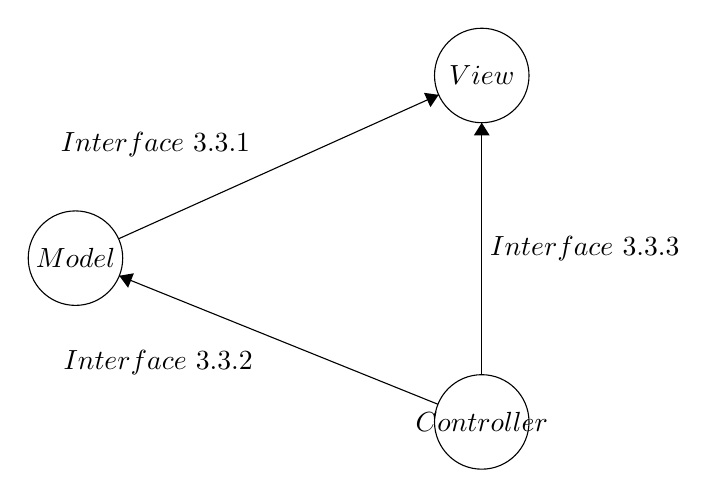
\begin{tikzpicture}[scale=0.2]
\tikzstyle{every node}+=[inner sep=0pt]
\draw [black] (39.5,-15.1) circle (3);
\draw (39.5,-15.1) node {$View$};
\draw [black] (13.7,-26.7) circle (3);
\draw (13.7,-26.7) node {$Model$};
\draw [black] (39.5,-37.1) circle (3);
\draw (39.5,-37.1) node {$Controller$};
\draw [black] (36.72,-35.98) -- (16.48,-27.82);
\fill [black] (16.48,-27.82) -- (17.04,-28.58) -- (17.41,-27.66);
\draw (18.95,-32.54) node [below] {$Interface\mbox{ }3.3.2$};
\draw [black] (16.44,-25.47) -- (36.76,-16.33);
\fill [black] (36.76,-16.33) -- (35.83,-16.2) -- (36.24,-17.11);
\draw (18.78,-20.32) node [above] {$Interface\mbox{ }3.3.1$};
\draw [black] (39.5,-34.1) -- (39.5,-18.1);
\fill [black] (39.5,-18.1) -- (39,-18.9) -- (40,-18.9);
\draw (40,-26.1) node [right] {$Interface\mbox{ }3.3.3$};
\end{tikzpicture}
\end{center}

\subsection{View Interface}

This is the View part of MVC (Model View Controller) design pattern. It holds all the classes that together builds the GUI of the application. The following are the classes and methods of all the classes inside view interface:

\subsubsection{FXApp}

It holds the main method of our application. Since we are using JAVAFx so we are initializing the BorderPane, Scene, Stage and then call the show method to run the application.

\subsubsection{FXController}

In this class we initialized the Left, Right, Center and Bottom part of the border pane. Below are the methods this class contains:

\begin{itemize}
	\item initialize(): It calls the four methods whenever a user opens the application. The four different methods are: initialLeftPart(), initialRightPart(), initialBottomPart(), initialCenterPart().
	\item initialCenterPart(): This is a table where the added food item gets listed. Every time user adds a food item the table gets updated.
	\item initialLeftPart(): The form to add a food item lyes here. We used grid pane to organize the form on the left side of the border pane. It also contains an event handler named addEventHandler. Here we distinguish the in dining and out dining serving. This 				handler also updates the data in the model of MVC so the list food display list always gets updated. Whenever user press the "Add Item" this handler gets triggered and update the display list in the centre and serving on the left side of the GUI.
	\item initialRightPart(): Items here are organized using grid pane. It has remove, Hide/Unhide Buttons and the list of "Total serving of Displayed item" and "Total serving of consumed items". Upon clicking the "Remove button" it does below things:
	\begin{itemize}
		\item Make sure the display list is not empty.
		\item Remove the selected food item from the table (Display table)
		\item Update the food group. If the removed item was the last item of that food group the set the colour of that food group to grey.
		\item Update the total serving of displayed items.
		\item Update the total serving of consumed items.
	\end{itemize}
	Upon clicking the "Hide/Unhide Consumed items" button:
	\begin{itemize}
		\item Check if the consumed items are already hidden. If so then update the diningManager to unhide them.
		\item If consumed items are not hidden then update the diningManager to hide consumed items.
		\item For each of the above change it will update the list of "Total serving of consumed items".
	\end{itemize}
	\item initialBottomPart(): We used HBox of JavaFx to organize the four buttons that updates food group.
	\item refreshItems(): Once the user add a food item by clicking the "Add Item" button this method clears out all the fields in for form on the left side of the GUI.
	\item stringToGroup(): Return the type of FoodGroup by the name of the food group selected by the user.
	\item markFoodGroupAdd(): There are four different counters, one for each Food Group to keep track how many food items belong to an individual group. This method increases that counter for an individual food group and sets the background colour green 				once a food has been added for a particular food group.
	\item markFoodGroupRemove(): It decreases the counter for a food group and sets the colour grey if there is no food listed in the display table.
	\item validateInput(TextField): Checks if the text fields are null or empty. If so then return false, else return true.
	\item validateInput(ComboBox): If the user did not select one food group from the drop down then it return false. Else it returns true.
	\item validateInput(DatePicker): If no date is selected then this method will return false. Else it will return true.
	\item validateInputServing(): Checks and validates the input for serving (Calories, Fat, Sodium and Sugar). It uses the validateInput(TextField) to make sure the fields are not null or empty. If not then it cast the value for each field from string to double.
	\item validateInputTime(): It uses the validateInput(TextField) to make sure the field is not null or empty. Then it parse the time into LocalTime format. If the input is not valid the method will display the placeholder to give the hind of the format to use to input time.
	\item validateInputIndining(): Using validateInput it checks all the field except retailer as it will not be useable for in dining. Returns true if all the fields have valid input else false.
	\item validateInputOutdining(): It does the same as validateInputIndining(). This method skips to check type as out dining does not have any type. Returns true if all the fields have valid input else false.
\end{itemize}

\subsubsection{DiningTableRow}

\begin{itemize}
	\item Constructor: Initialize checkbox. Sets an action on checkbox. It updates the diningManager (Where the data is stored) and also the Consume serving upon selecting or deselecting the checkbox.
\end{itemize}
\subsection{Model Interface}
The Model portion of the MVC (Model View Controller) design architecture. Every class in this module will be instanced as an object to store the necessary data for the application. Below are the detailed specifications of the classes.

\subsubsection{Dining}
The parent class to both Indining and Outdining. The main object type that is used to store data for the user food items.
\begin{itemize}
\item Dining(): Constructor for the Dining class.
\item getName(): Accessor method for name variable.
\item setName(): Mutator method for name variable.
\item getFoodGroup(): Accessor method for foodGroup variable.
\item setFoodGroup(): Mutator method for foodGroup variable.
\item getServing(): Accessor method for serving variable.
\item setServing(): Mutator method for serving variable.
\item getMeal): Accessor method for meal variable.
\item setMeal(): Mutator method for meal variable.
\item isConsumed(): Accessor method for consumed variable.
\item setConsumed(): Mutator method for consumed variable.
\end{itemize}

\subsubsection{Indining}
Subclass of the Dining class.

\begin{itemize}
\item Indining(): Constructor of the Indining class.
\item getType(): Accessor of the type variable.
\item setType(): Mutator of the type variable.
\item toString(): Returns String object containing information for the name and consumed variables.
\item equals(): Method that determines if the passed argument object is equal to the calling object.
\item hashCode(): Method to create and return a hash code for Indining object.
\end{itemize}

\subsubsection{Outdining}
Subclass of the Dining class.

\begin{itemize}
\item Outdining(): Constructor for the Outdining class
\item getRetailer(): Accessor for the retailer variable.
\item setRetailer(): Mutator for the retailer variable.
 \item toString(): Returns String object containing information for the name and consumed variables.
 \item equals(): Method that determines if the passed argument object is equal to the calling object.
 \item hashCode(): Method to create and return a hash code for Out dining object.
\end{itemize}

\subsubsection{Serving}
Class that records the data related to nutritional content of food items.
\begin{itemize}
\item Serving(): Constructor for the Serving class.
\item getAmount(): Accessor for the amount variable.
\item setAmount(): Mutator for the amount variable.
\item getCalories(): Accessor for the calories variable.
\item setCalories(): Mutator for the calories variable.
\item getFat(): Accessor for the fat variable.
\item setFat(): Mutator for the fat variable.
\item getSodium(): Accessor for the sodium variable.
\item setSodium(): Mutator for the sodium variable.
\item getSugar(): Accessor for the sugar variable.
\item setSugar(): Mutator for the sugar variable.
 \item equals(): Method that determines if the passed argument object is equal to the calling object.
 \item hashCode(): Method to create and return a hash code for Serving object.
 \item toString(): Method that returns all of the stored data for each variable of the Serving class as a String object.
\end{itemize}

\subsection{Controller Interface}

The class is called DiningManager. To store the data we used an array. There is an observer to observe the changes happened by any interaction from the user using the GUI. Below are the methods it contains:

\begin{itemize}
	\item addDiningItem(): This method initialize an instance of DiningTableRow class. Notify the observer and updates the array list of table that displays the food items. Calls this method addDiningItemDataModel() which will be described below.
	\item addDiningItemDataModel(): Updates the array list that contains all the data.
	\item removeDiningItem(): Checks if the collection is not empty. Then remove the selected item from Dining Item. Check if the array list for dining table is empty. If not then remove the selected item from dining item. At the end calls the below method.
	\item removeDiningItemDataModel(): Checks if the array list for all the dining item is empty. If not then remove the selected item from array list.
	\item markConsumed(): Iterate through all the dining item in the dining table and sets the value true for all the items that the user selected consumed for. Then calls the below method.
	\item markConsumedDataModel(): Gets the index number of the item the user selected as consumed and update the array list of data.
	\item markUnConsumed(): Iterate through all the dining item in the dining table and sets the value false for all the items that the user deselected consumed for.
	\item hideConsumed(): If the item is in the collection (Observer) the this method removes it.
	\item unHideConsumed(): Iterate through all the items in the dining table array list and if the item does not exist in the collection the adds it.
	\item updateCurrServing(): Iterate all the dining table row in the array list and updates the serving for each of then and then updates the total.
\end{itemize}

\section{Domain Model}

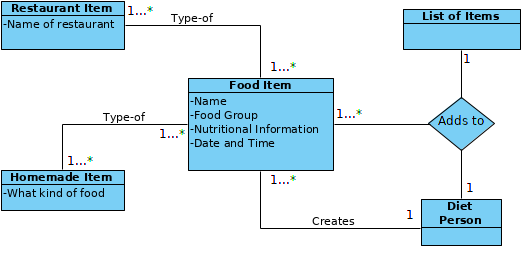
\includegraphics[width=11cm]{pictures/Domain-Diagram.png}

This domain model abstracts the concepts required to formulate the design of the personal dietary application. They are used as a guide to build classes which make up the modules of the program. The main actor, the Diet Person, is the user of the application. This entity will be keeping track of various food items and their nutritional information on an electronic list. This person can either eat professionally made restaurant food items or prepare produce and various sustenance at their dwelling. The application will need to keep track of this data.

\section{Class Diagrams}

The Personal Dietary Application outlined in this design document consists of three main folders containing the source files of classes. Their makeup is transcribed as UML diagrams in the following subsections. Regarding software architecture and design patterns, the classes adhere to the Observable-Observer pattern by making use of the ObservableList objects available from the JavaFX library. The Model-View-Controller (MVC) architecture is paired with this Observable implementation by mediating the tasks of model, view, and controller among the three folders. Inside the GUI folder, there is also another controller to handle event captures from the user interface. \par
GRASP principles are practiced by having the DiningTableRow class in the GUI Folder operate as the information expert. The class contains all of the stored data related to the items input by the user and allows retrieval and creation of these objects. The FXController functions as the GRASP controller to receive and manipulate events, acting as an event listener.

\subsection{GUI Folder (View)}

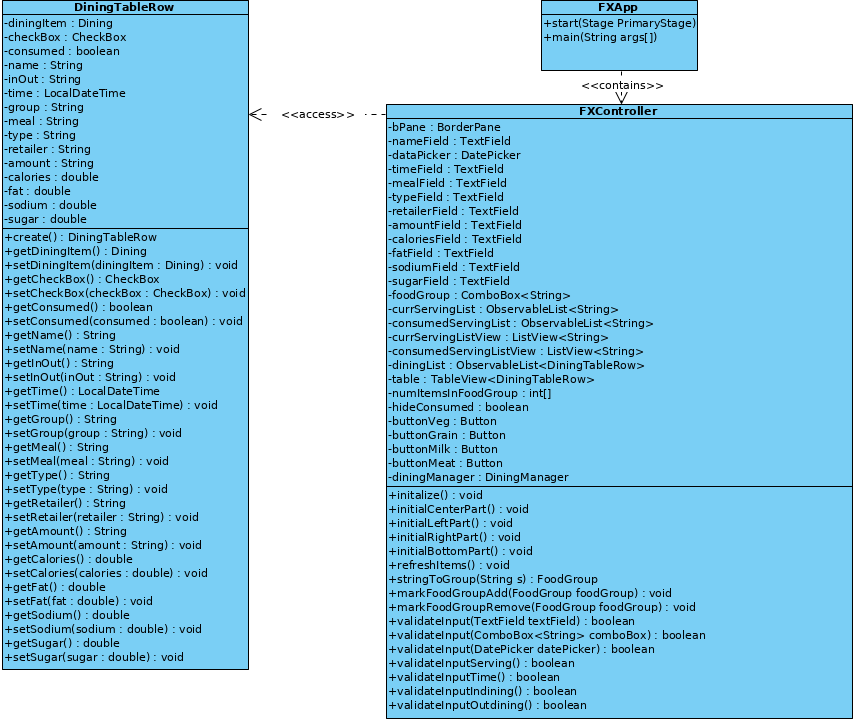
\includegraphics[width=17cm]{pictures/GUI-Class-Diagram.png}

\subsection{bean Folder (Model)}

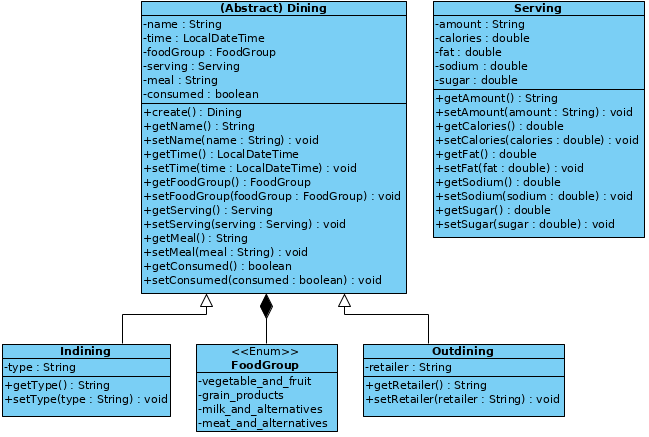
\includegraphics{pictures/Bean-Class-Diagram.png}

\subsection{business folder (Controller)}

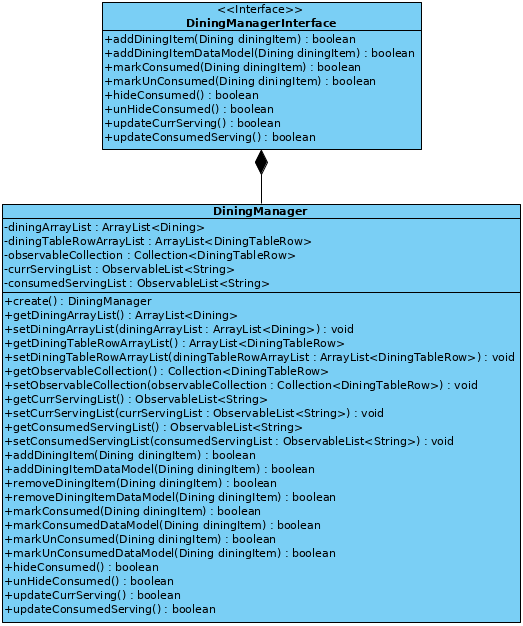
\includegraphics{pictures/Business-Class-Diagram.png}

\chapter{Dynamic Sequence Diagrams of the Interface}

We have selected to use sequence diagrams to better understand the communication between different classes and their methods. Below are the major functionalities of our application:

\section{Launch Application}

\begin{figure}[!htbp]
\centering
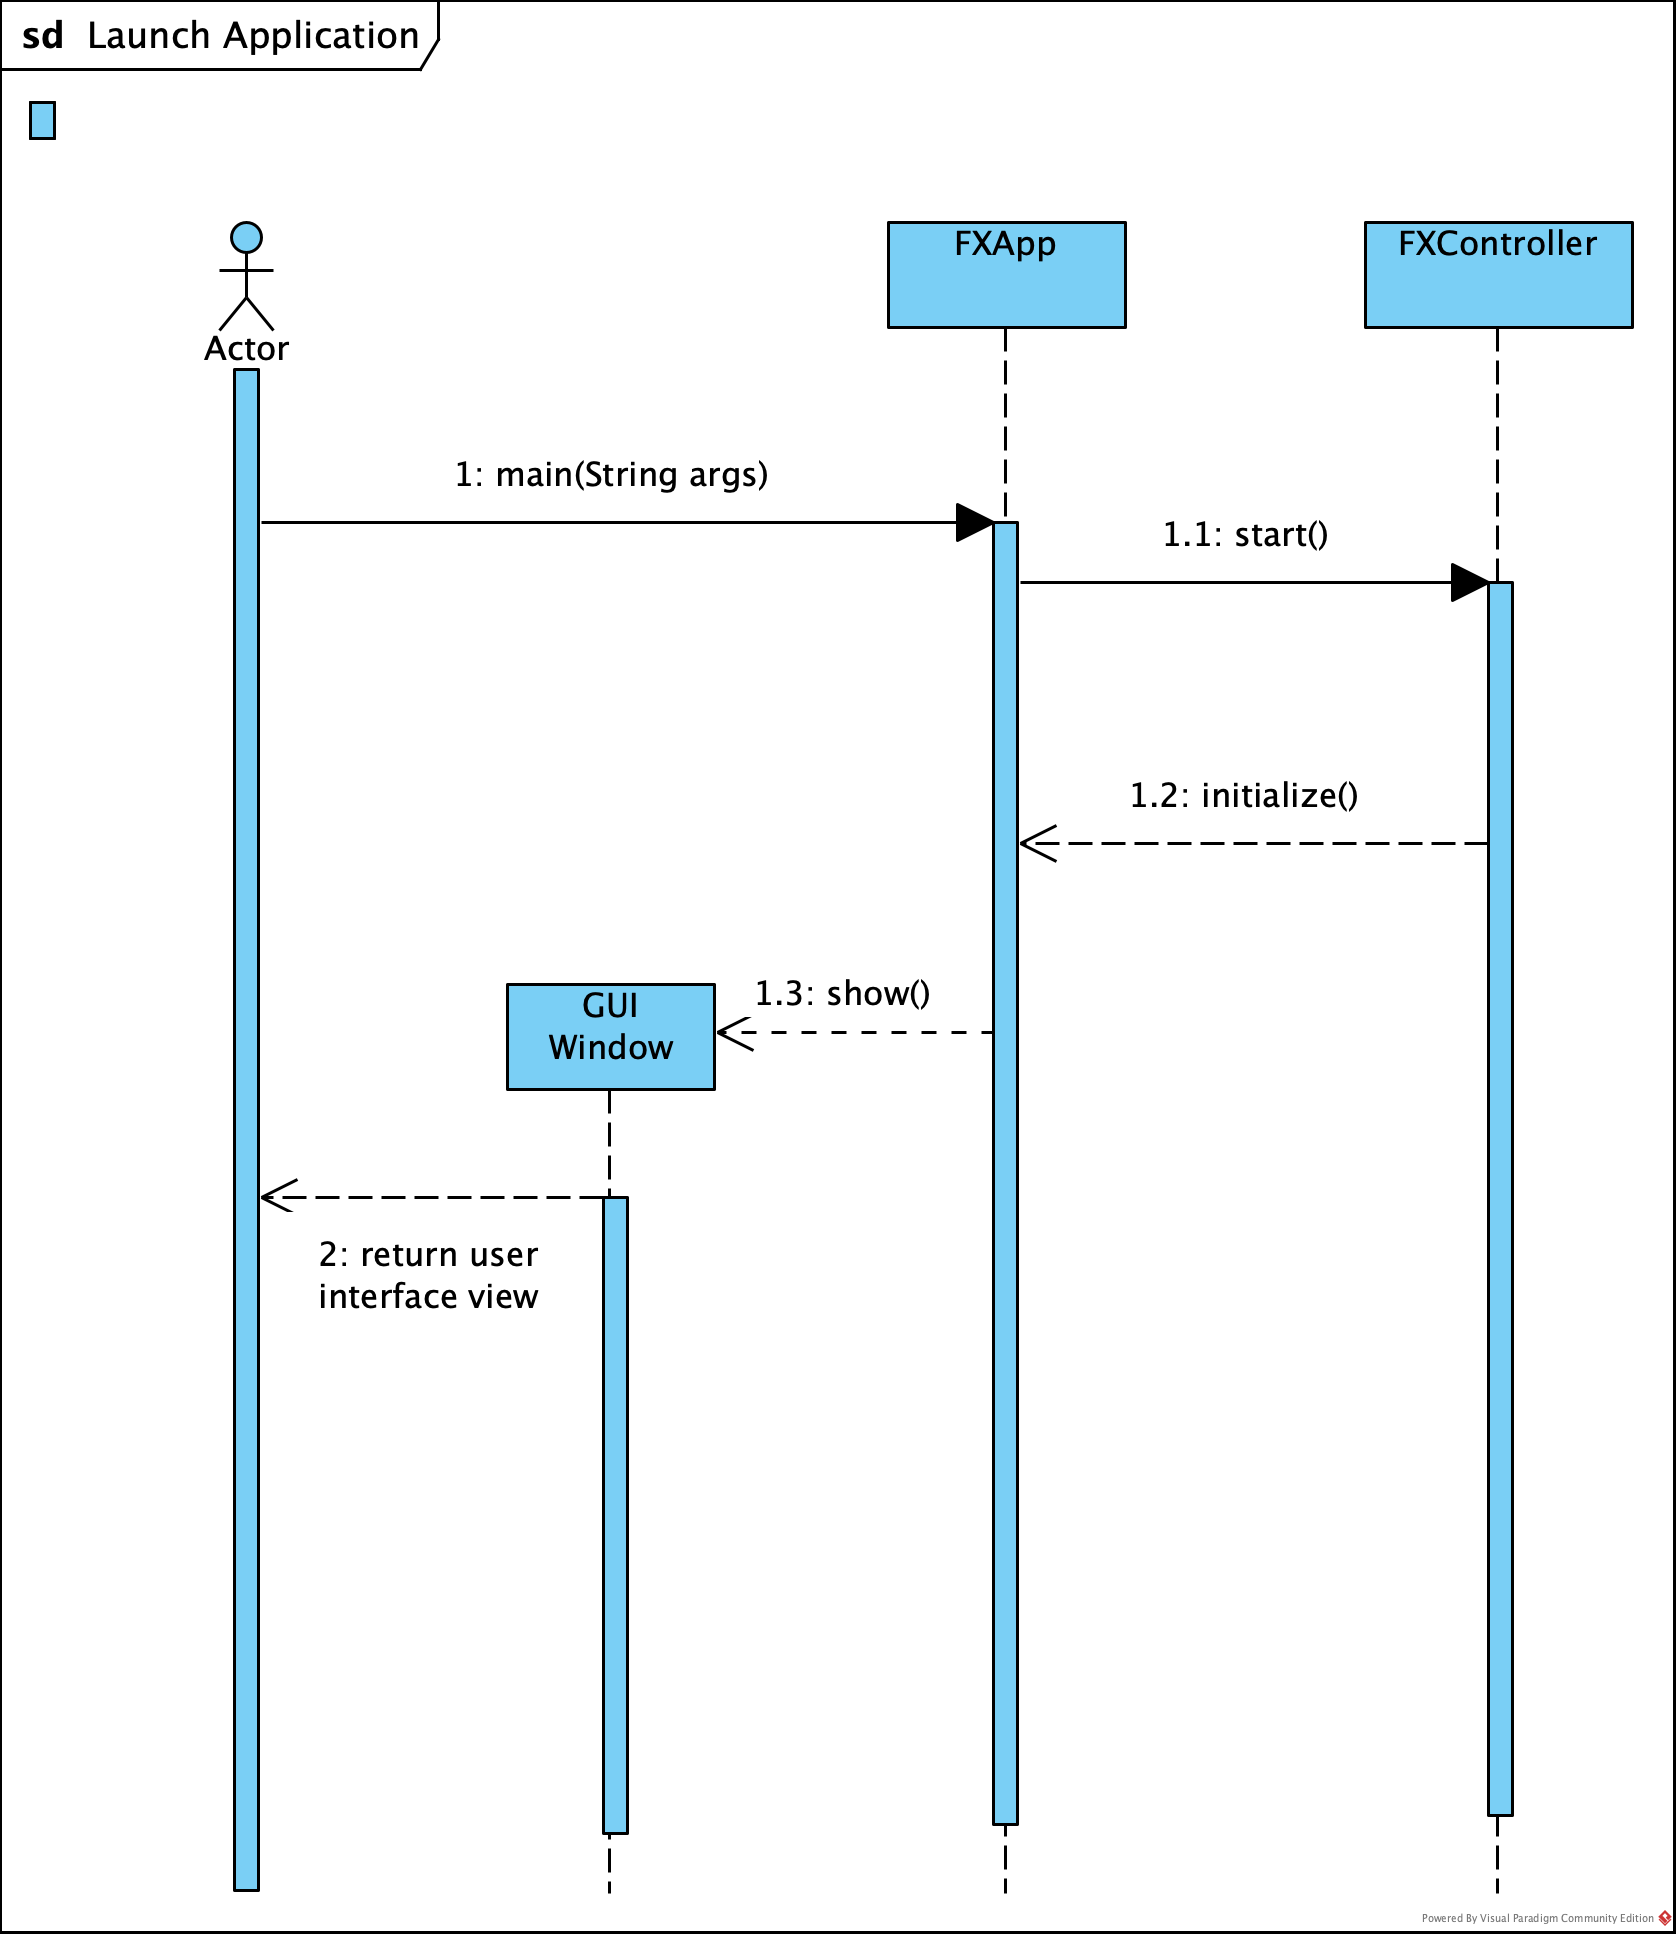
\includegraphics[width=10.8cm]{pictures/sd-LaunchApp.png}
\caption{Sequence Diagram of Launching the Application}
\end{figure}

\FloatBarrier

\section{Add a food item}

The following diagram pictures the scenario when a user clicks the Add Item button. First the data will be collected from the form and it will be added into the Dining table (Model) and also the serving will be updated. The food group will also be coloured to indicate a specific food has been consumed.

\begin{figure}[!htbp]
\centering
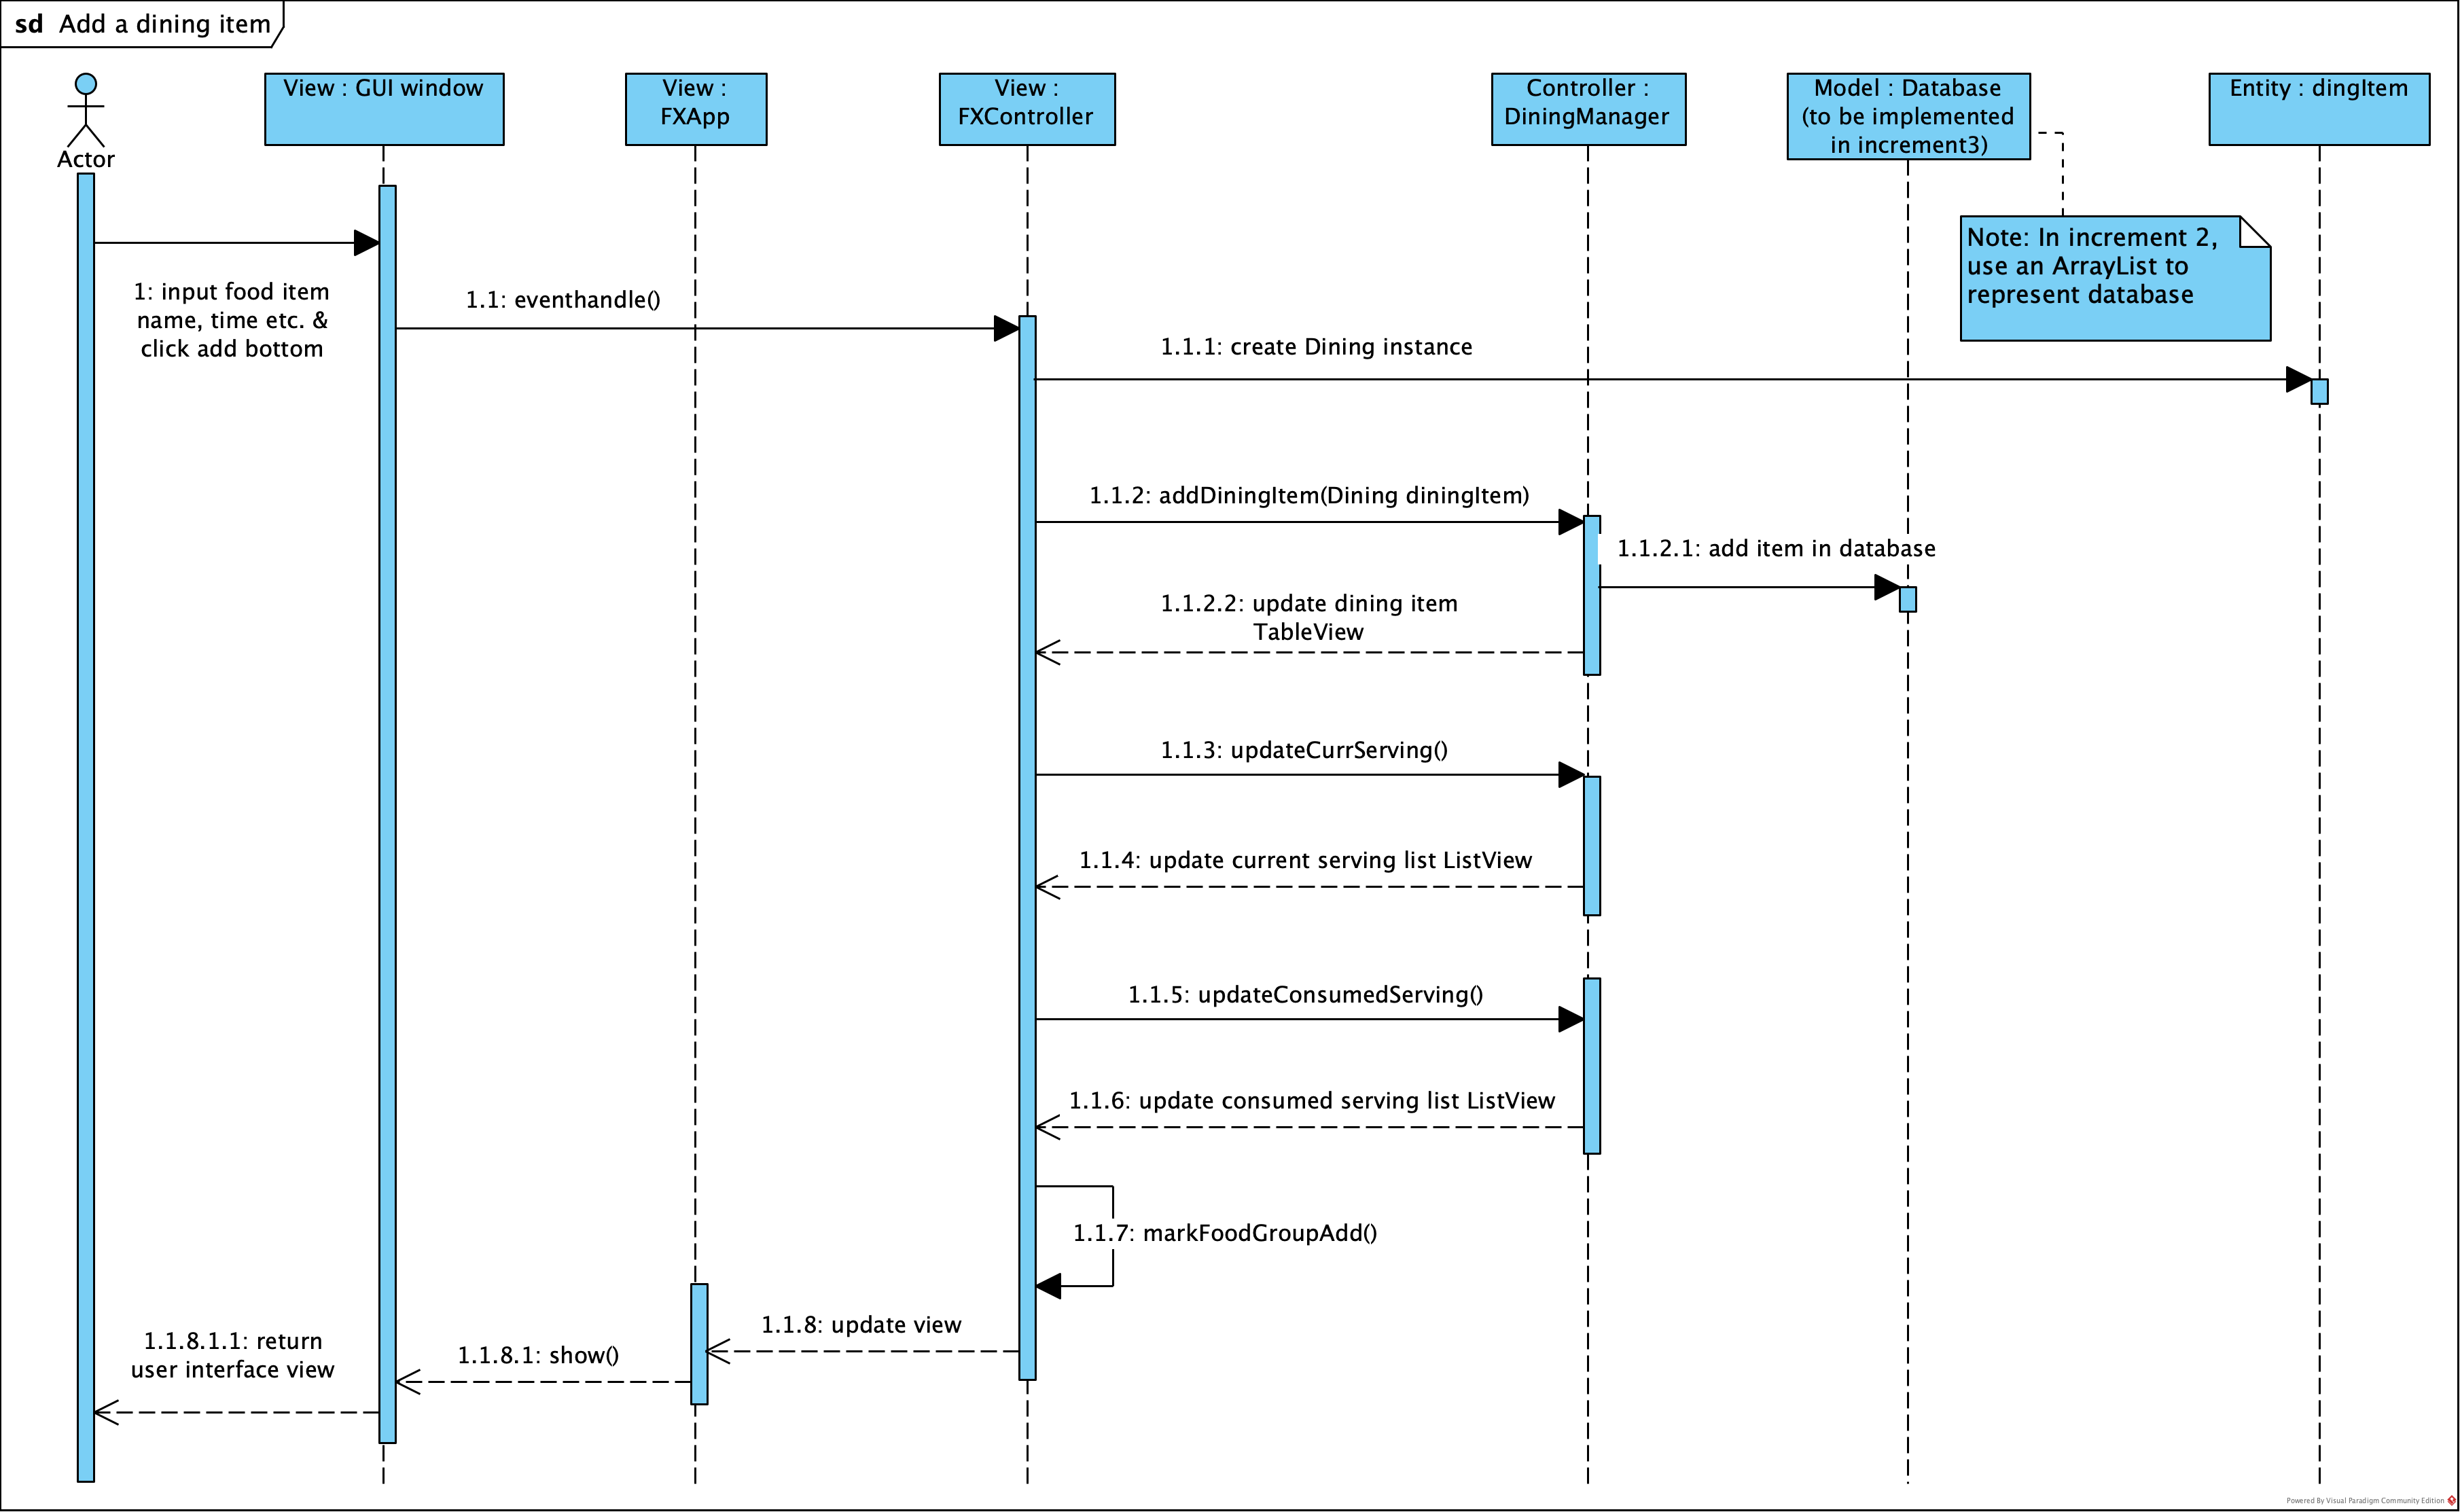
\includegraphics[width=17.5cm]{pictures/sd-addItem.png}
\caption{Sequence Diagram of adding a food item}
\end{figure}

\FloatBarrier

\newpage

\section{Remove a food item}

The following diagram displays the process for user to remove a food item. It will update the display table followed by dining manager. Also it will check the food group to make sure there are food available in the list for a particular food group.
\begin{figure}[!htbp]
\centering
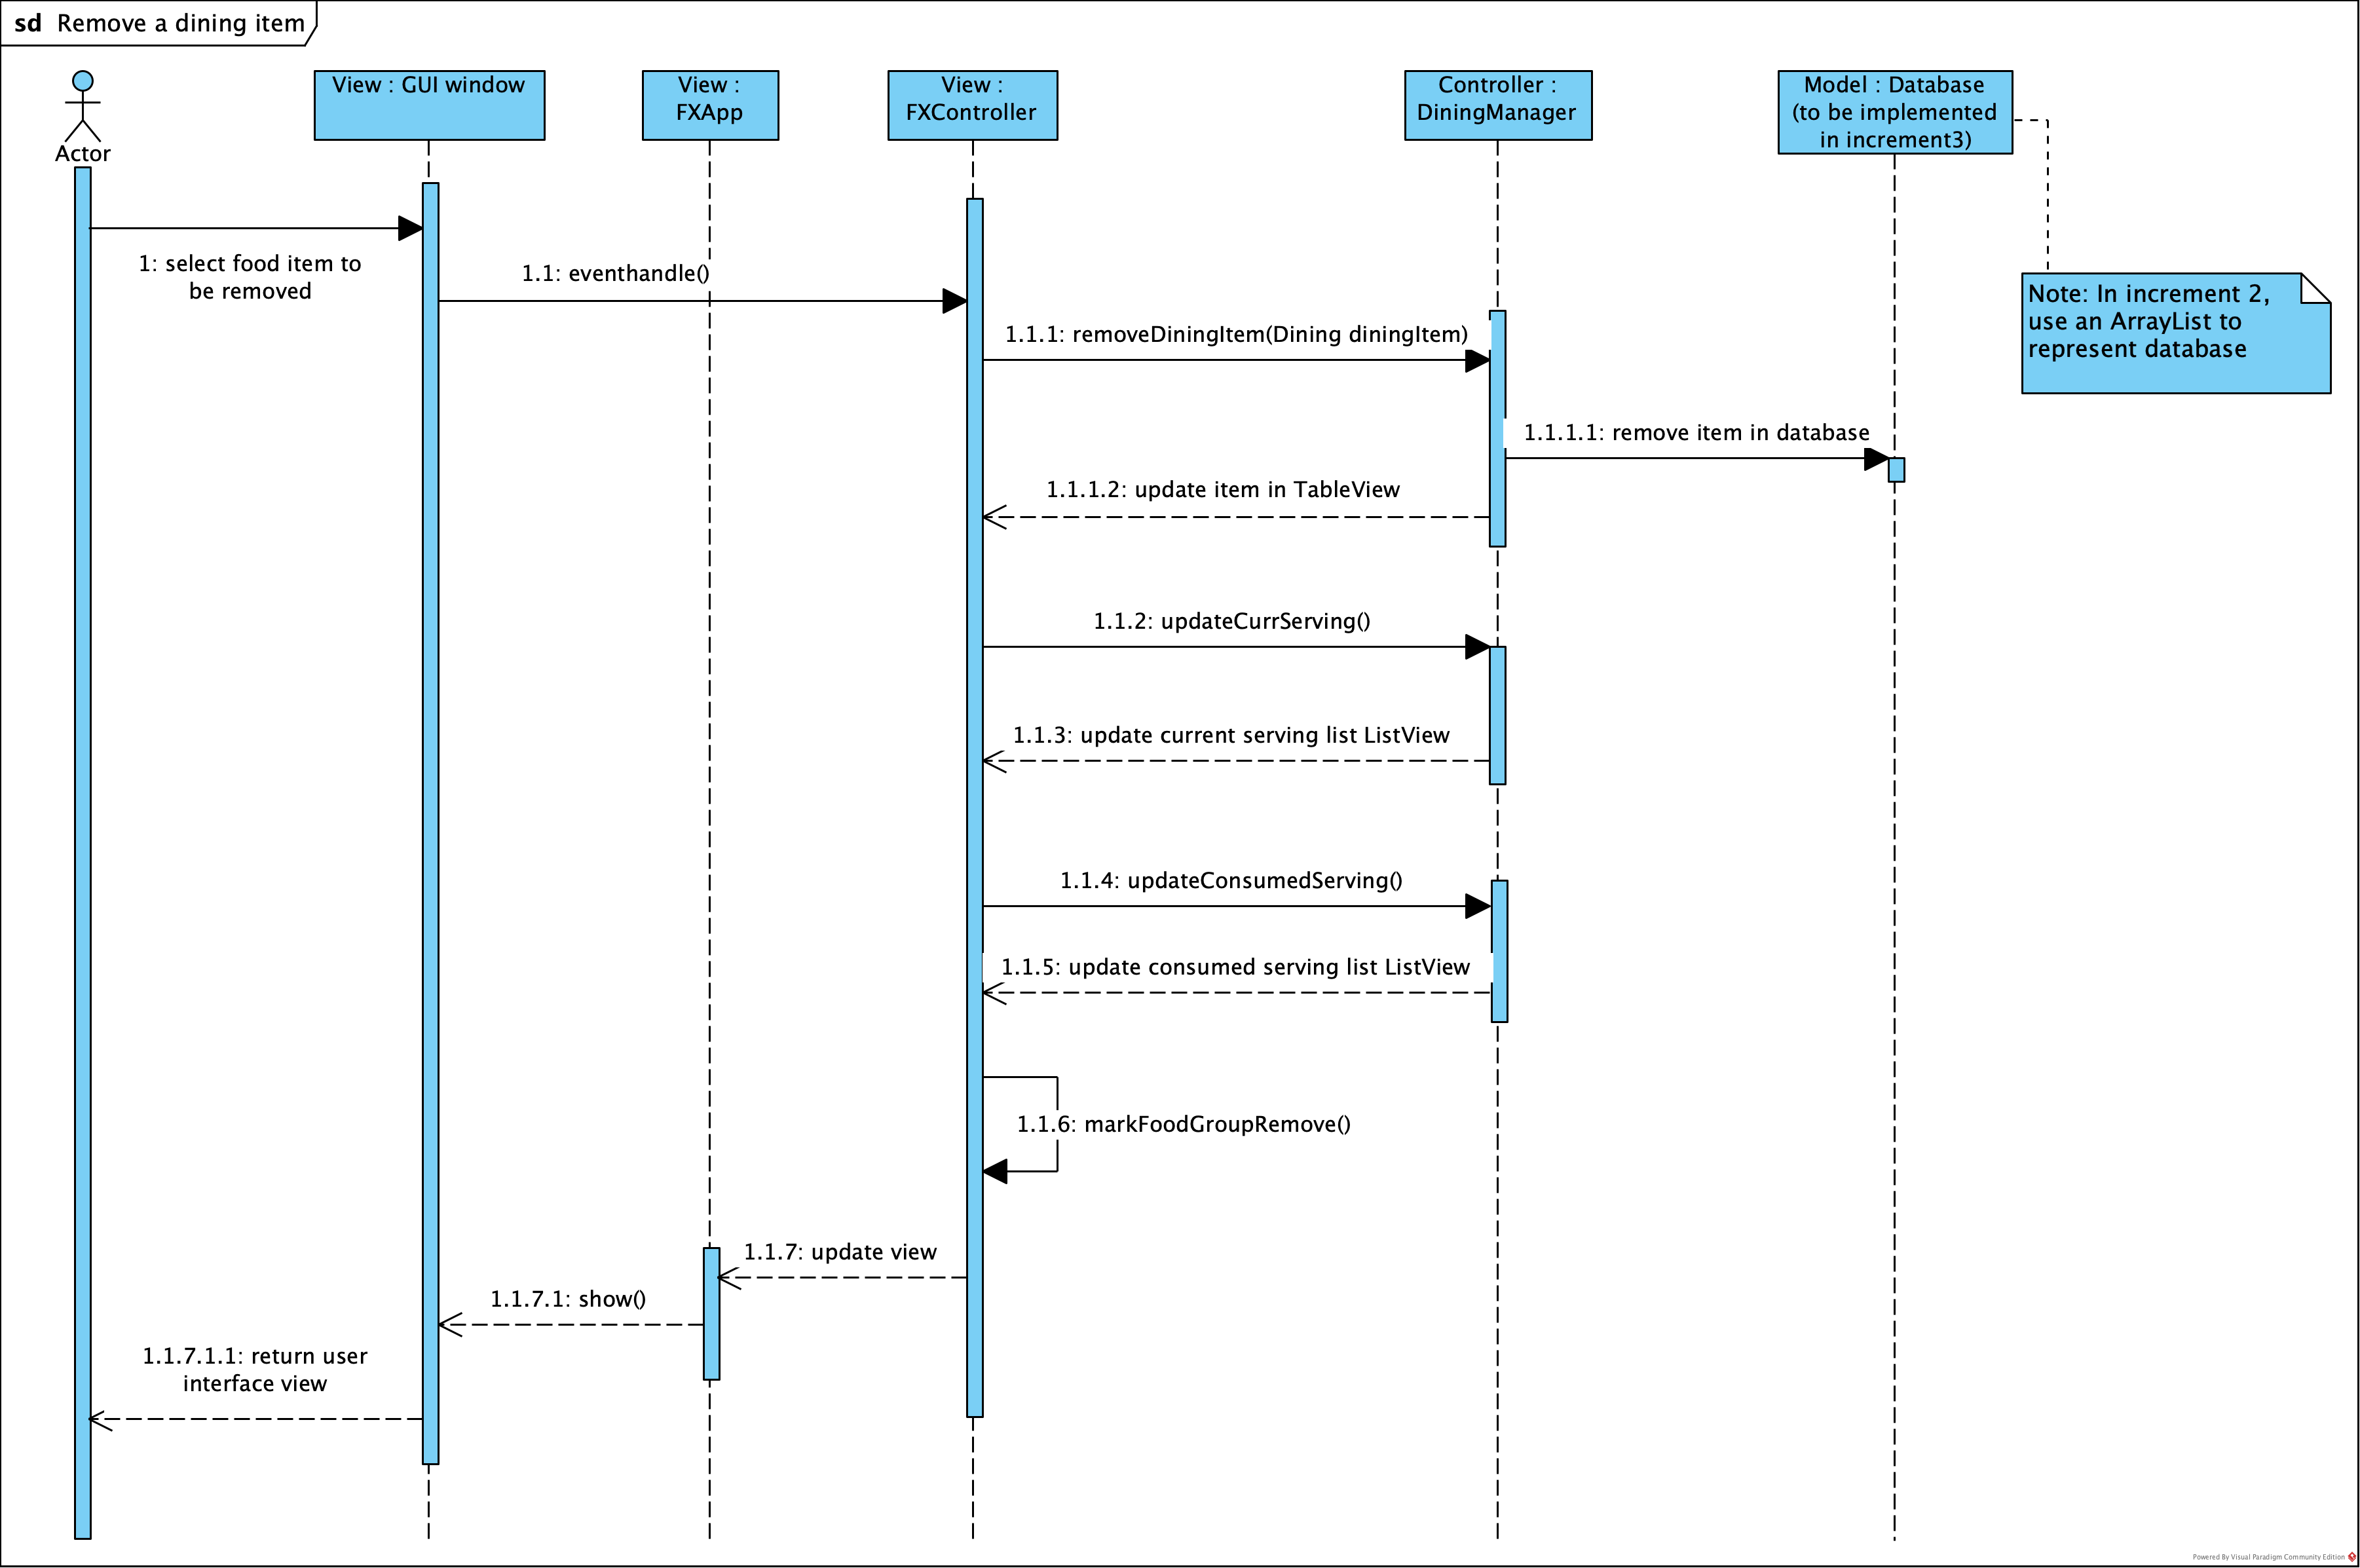
\includegraphics[width=17.5cm]{pictures/sd-removeItem.png}
\caption{Sequence Diagram of removing a food item}
\end{figure}

\FloatBarrier

\newpage

\section{Mark as consumed}

The following diagram illustrates the option to mark an added food item as consumed or not-consumed. There is an event handler in the DiningTableRow class which will update the DiningManager class.

\begin{figure}[!htbp]
\centering
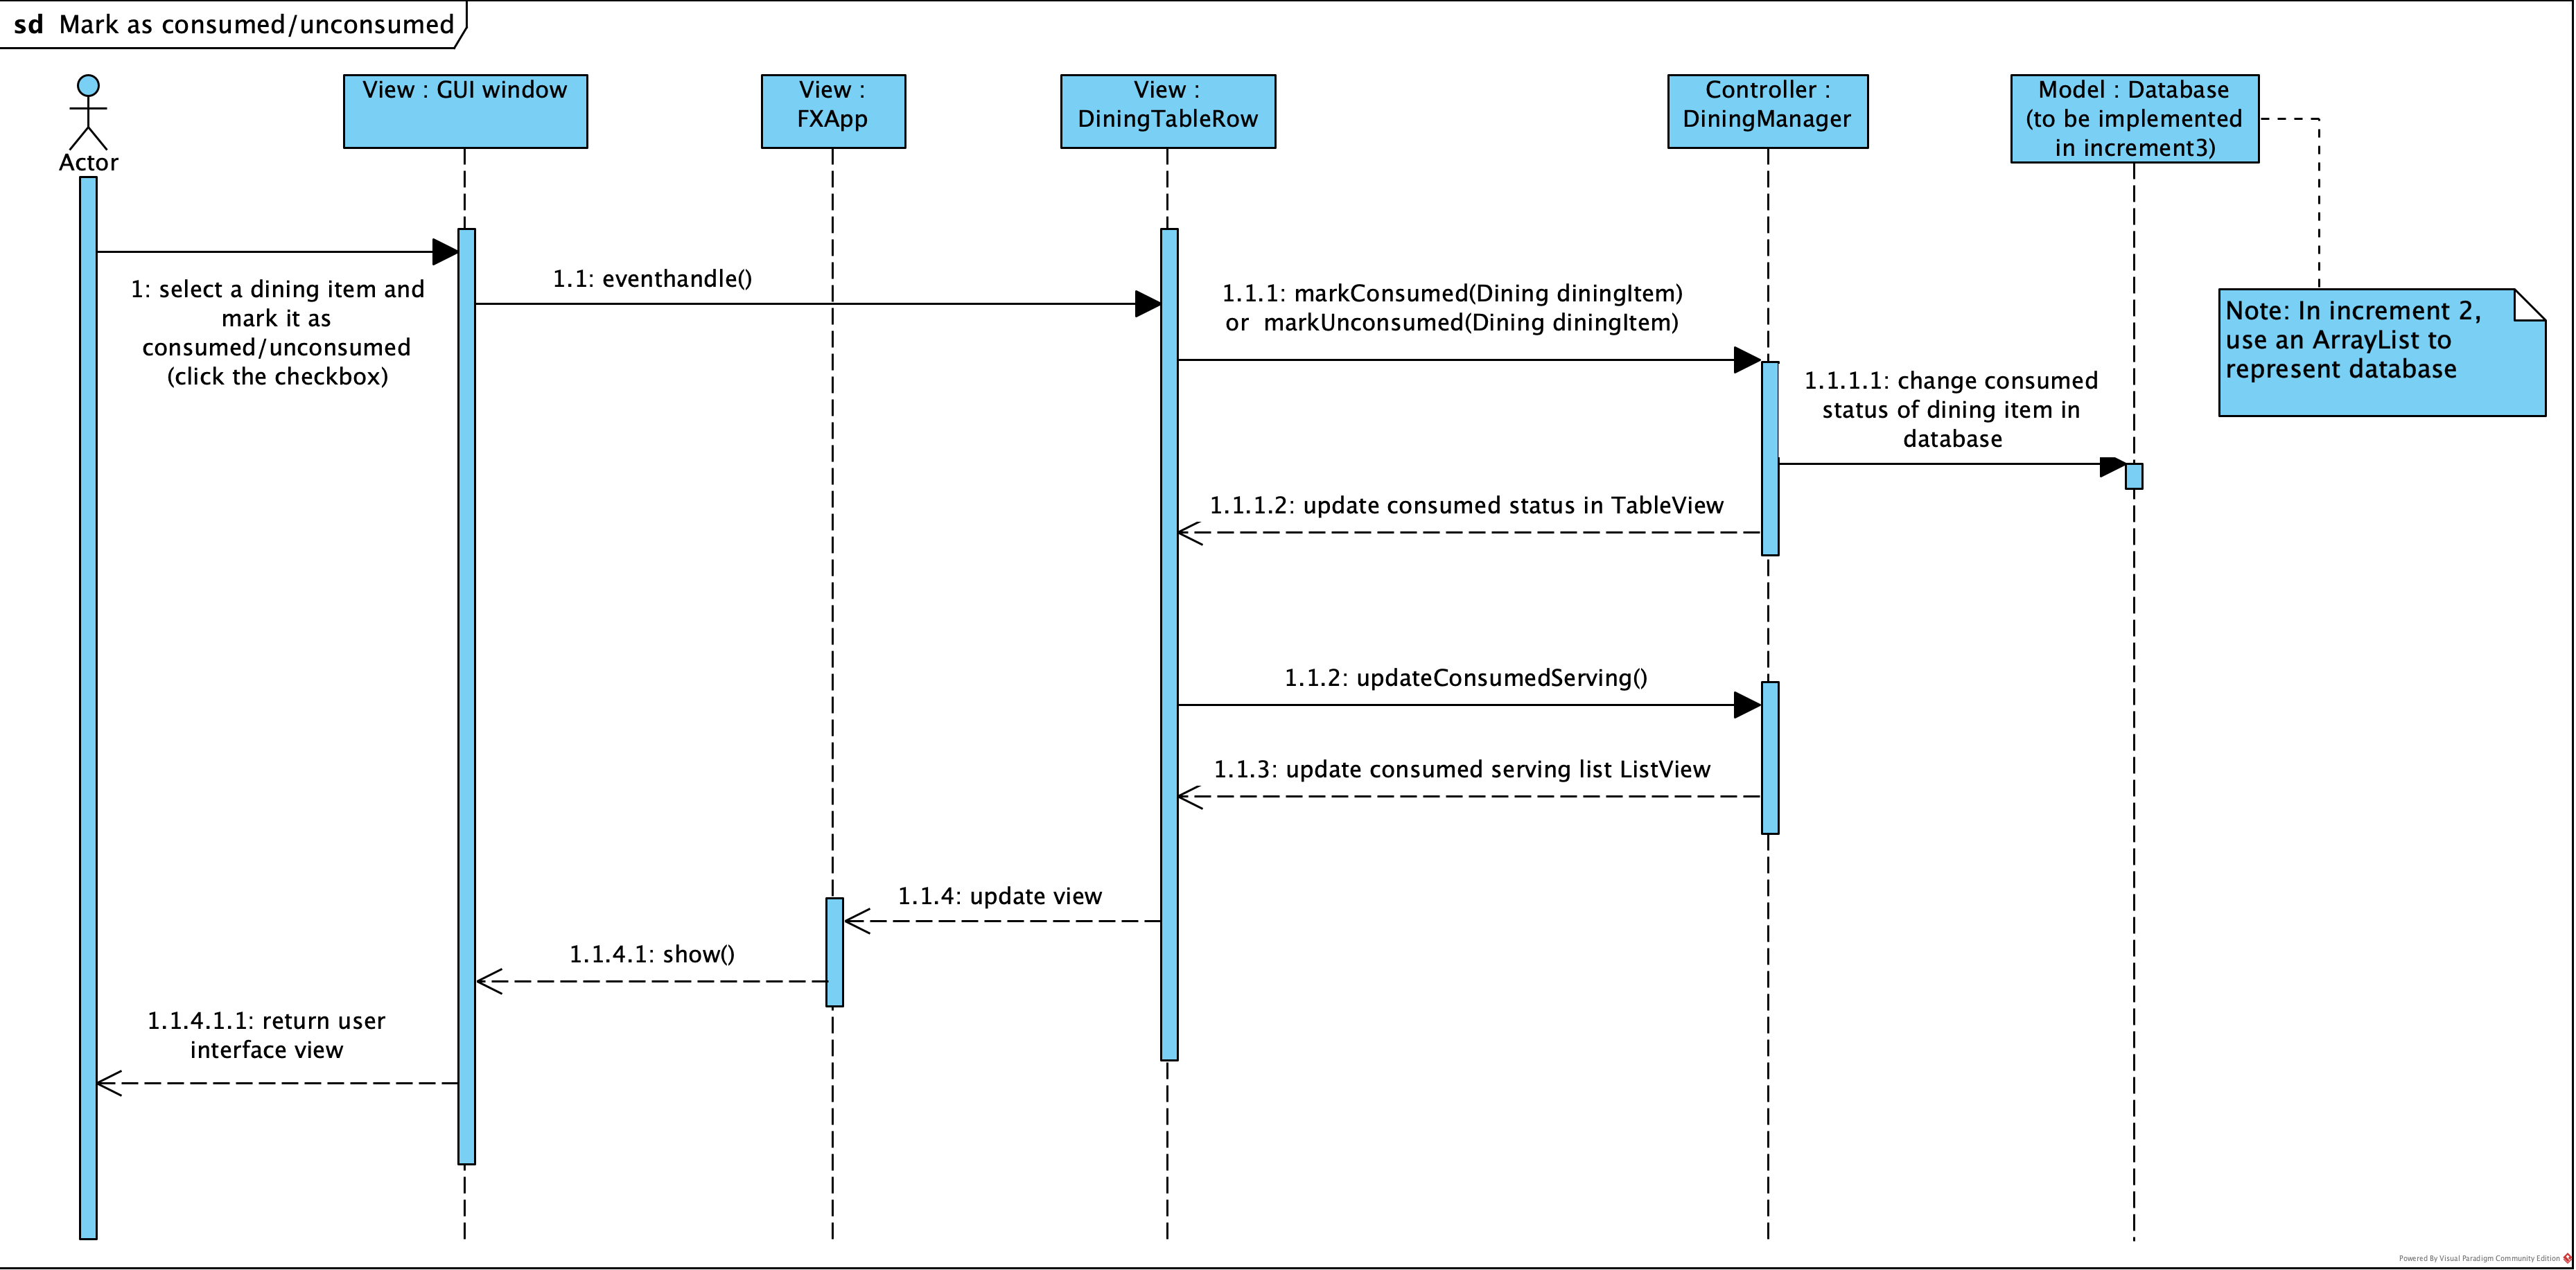
\includegraphics[width=17.5cm]{pictures/sd-markConsumed.png}
\caption{Sequence Diagram of marking food items as consumed or not-consumed}
\end{figure}

\FloatBarrier

\newpage

\section{Hide/Unhide an added food item}

The following diagram shows the sequence to hide/unhide a food item. It will  update three methods in the diningManager class (unHideConsumed(), hideConsumed(), updateServing()).

\begin{figure}[!htbp]
\centering
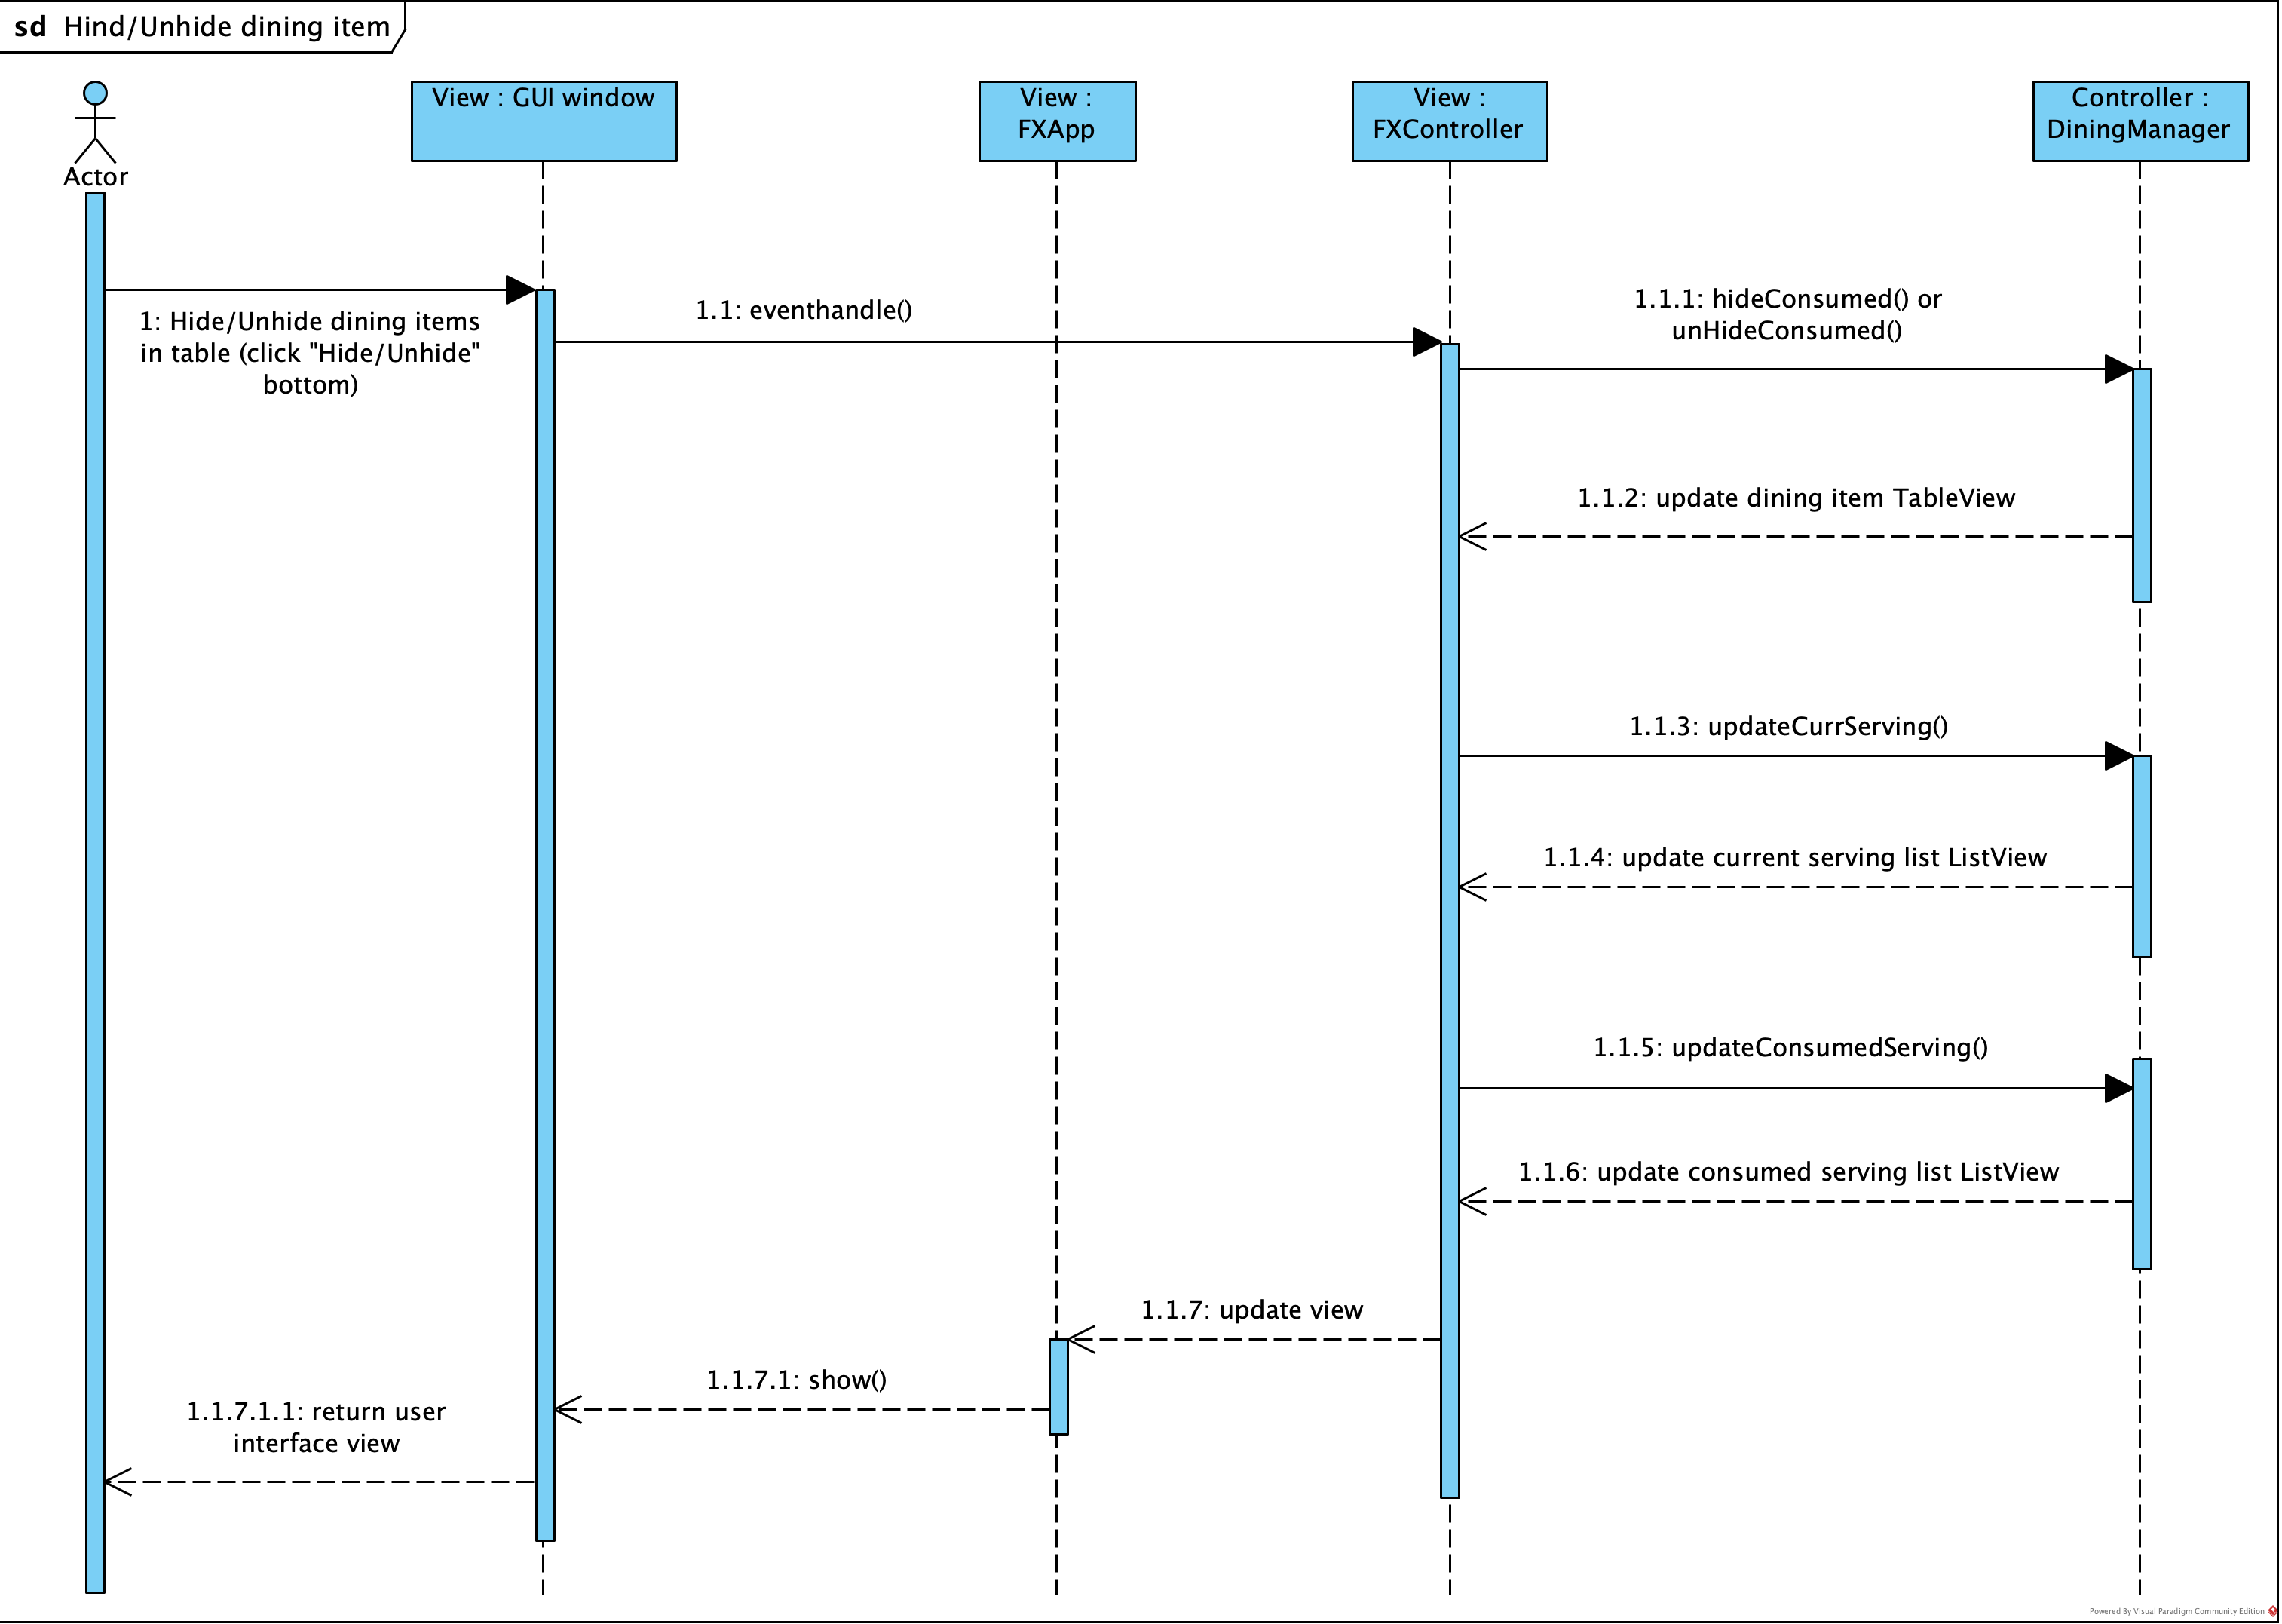
\includegraphics[width=17.5cm]{pictures/sd-hideConsumed.png}
\caption{Sequence Diagram of hiding unhiding consumed item(s)}
\end{figure}

\FloatBarrier

\end{document}
